% Split Eigen-analysis and Complex Arithmetic into two chapters
\chapter{Eigen-analysis}
\label{ch_eig}

\section{Eigenvalues and eigenvectors}

\begin{definition}
Let $A$ be an $n\times n$ matrix. A number $\lambda$ and a vector
$\xx$ are called an eigenvalue eigenvector pair if
\begin{enumerate}[(1)]
\item $\xx\ne\zv$ 
\item $A\xx = \lambda\xx$ 
\end{enumerate}
\end{definition}

In other words, the action of $A$ on the vector $\xx$ is to stretch or
shrink it by an amount $\lambda$ without changing its direction. We
say $\lambda$ is an eigenvalue of $A$ if there exists a vector $\xx$
so that $\lambda$ and $\xx$ are an eigenvalue eigenvector pair.
Notice that we do not allow $\xx=\zv$. If we did, any number $\lambda$
would be an eigenvalue. However we do allow $\lambda=0$. Saying that
$0$ is an eigenvalue of $A$ means that there is a non-zero solution
$\xx$ (the eigenvector) of $A\xx=0\xx=\zv$. So we see that $0$ is an
eigenvalue of $A$ precisely when $A$ is not invertible.

Let's look at some examples.  Consider first the matrix of reflection
about a line making an angle of $\theta$ with the $x$ axis shown in
Figure~\ref{fig_refeig}.  Let $\xx$ be any vector that lies along the
line. Then the reflection doesn't affect $\xx$. This means that $R\xx
= \xx$. In other words, $\xx$ is an eigenvector with eigenvalue $1$. On
the other hand, suppose that $\yy$ is a vector at right angles to the
line. Then the reflection flips $\yy$ into minus itself. So
$R\yy=-\yy$.  In other words, $\yy$ is an eigenvector with eigenvalue
$-1$. If we take any other vector and reflect it, we don't end up with
a vector that lies on the same line as the original vector. Thus there
are no further eigenvectors or eigenvalues.

\begin{figure}
\centerline{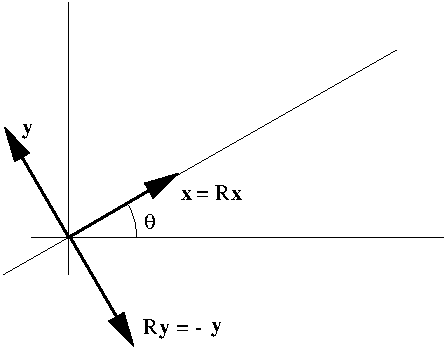
\includegraphics[height=1.5in]{5_refeig}}
\caption{Eigenvalues and eigenvectors of a 2D reflection. 
\label{fig_refeig}}
\end{figure}

An important point to notice is that the eigenvector is not uniquely
determined.  The vector $\xx$ could be {\it any} vector along the
line, and $\yy$ could be {\it any} vector orthogonal to the line. In
fact, if we go back to the original definition of eigenvalue and
eigenvector we can see that if $\lambda$ and $\xx$ are an eigenvalue
eigenvector pair, then so are $\lambda$ and $s\xx$ for any non-zero
number $s$, since $s\xx\ne\zv$ and $As\xx=sA\xx=s\lambda \xx =\lambda
s\xx$. So the important thing about an eigenvector is its direction,
not its length. However, there is no such ambiguity in the definition
of the eigenvalue. The reflection matrix has exactly two eigenvalues:
$1$ and $-1$.

In some sense, the reflection matrix $R$ illustrates the most
satisfactory situation. $R$ is a $2\times 2$ matrix with two distinct
eigenvalues. The corresponding eigenvectors $\xx$ and $\yy$ are
linearly independent (in fact they are orthogonal) and form a basis
for two dimensional space.  It will be important in applications to
determine whether or not there exists a basis of eigenvectors of a
given matrix. In this example, $\xx$ and $\yy$ are a basis of
eigenvectors of $R$.

As our next example, consider the identity matrix $I$. Since the
identity matrix doesn't change a vector, we have $I\xx=\xx$ for any
vector $\xx$.  Thus any vector $\xx$ is an eigenvector of $I$ with
eigenvalue $1$.  This example shows that a given eigenvalue may have
many eigenvectors associated with it. However, in this example, there
still exists a basis of eigenvectors: any basis at all is a basis of
eigenvectors of $I$.

Next we will consider the rotation matrix $\ldots$ and run into
trouble. Suppose $R$ is the matrix of rotation by $\pi/4$ ({\em i.e.}
$45^\circ$). Then $R\xx$ is never in the same direction as $\xx$,
since $R$ changes the direction of $\xx$ by $\pi/4$. So $R$ has no
eigenvalues and no eigenvectors. This unfortunate state of affairs
will cause us to make a considerable detour into the theory of complex
numbers. It turns out that if we work with complex numbers rather than
real numbers, then the rotation matrix has eigenvalues too.

\subsection{Computing the eigenvalues and eigenvectors}

We now consider the problem of finding all eigenvalue eigenvector
pairs for a given $n\times n$ matrix $A$. To start, suppose someone
tells you that a particular value $\lambda$ is an eigenvalue of
$A$. How can you find the corresponding eigenvector $\xx$?  This
amounts to solving the equation $A\xx=\lambda\xx$ for $\xx$. This can
be rewritten
\[
(A-\lambda I)\xx = \zv,
\]
where $I$ denotes the identity matrix. In other words $\xx$ is a
non-zero solution to a homogeneous equation. It can be found by
Gaussian elimination.

For example, suppose you know that $4$ is an eigenvalue of
\[
\left[\matrix{3&-6&-7\cr 1&8&5\cr -1& -2 & 1\cr}\right].
\]
To find the corresponding eigenvector, we must solve
\[
\left(\left[\matrix{3&-6&-7\cr 1&8&5\cr -1& -2 & 1\cr}\right] 
- 4\left[\matrix{1&0&0\cr 0&1&0\cr 0& 0& 1\cr}\right]\right)
\left[\matrix{x_1\cr x_2\cr x_3\cr}\right] = 
\left[\matrix{0\cr 0\cr 0\cr}\right].
\]
This can be written
\[
\left[\matrix{-1&-6&-7\cr 1&4&5\cr -1& -2 & -3\cr}\right]
\left[\matrix{x_1\cr x_2\cr x_3\cr}\right] = 
\left[\matrix{0\cr 0\cr 0\cr}\right].
\]
To solve this we reduce the matrix. This yields
\[
\left[\matrix{-1&-6&-7\cr 0&-2&-2\cr 0&0&0\cr}\right]
\]
The fact that the rank of this matrix is less than $3$ confirms that
$4$ is indeed an eigenvalue. If the rank of the matrix were $3$ then
the only solution to the equation would be $\zv$ which is not a valid
eigenvector.

Taking $x_3=s$ as a parameter, we find that $x_2=-s$ and
$x_1=-s$. Thus
\[
\xx = s\left[\matrix{-1\cr -1\cr 1\cr}\right]
\]
is an eigenvector (for any non-zero choice of $s$). In particular, we
could take $s=1$. Then
\[
\xx = \left[\matrix{-1\cr -1\cr 1\cr}\right].
\]
When doing calculations by hand, it makes sense to take the scalar 
multiple $s$ in the eigenvector calculation so that it simplifies the 
form of the eigenvector (clears common denominators in the components, for example).
Eigenvectors computed in MATLAB  are normalized (scaled so that they 
have length 1). 

Now that we have a method for finding the eigenvectors once we know
the eigenvalues, the natural question is: Is there a way to determine
the eigenvalues without knowing the eigenvectors? This is where
determinants come in.  The number $\lambda$ is an eigenvector if there
is some non-zero solution $\xx$ to the equation $(A-\lambda
I)\xx=\zv$. In other words, $\lambda$ is an eigenvalue if the matrix
$(A-\lambda I)$ is not invertible.  This happens precisely when
$\det(A-\lambda I)=0$.

This gives us a method for finding the eigenvalues. Compute
$\det(A-\lambda I)$.  This will be a polynomial in $\lambda$. The
eigenvalues will be exactly the values of $\lambda$ that make this
polynomial zero, i.e., the roots of the polynomial.

So here is the algorithm for finding the eigenvalues and eigenvectors:
\begin{enumerate}[(1)]
\item Compute $\det(A-\lambda I)$ and find the values of $\lambda$ for
which it is zero. These are the eigenvalues.
\item For each eigenvalue, find the non-zero solutions to $(A-\lambda
I)\xx=\zv$. These are the eigenvectors.
\end{enumerate}

I should mention that this is actually only a practical way to find
eigenvalues when the matrix is small. Finding eigenvalues of large
matrices is an important problem and many efficient methods have been
developed for use on computers.

\begin{example} Find the eigenvalues and eigenvectors of 
\[
A=\left[\matrix{2&1\cr 1&2\cr}\right].
\]
{\rm First we compute 
\begin{eqnarray*}
\det(A-\lambda I) &=& (2-\lambda)(2-\lambda)-1 \\
&=&\lambda^2 - 4\lambda +3
\end{eqnarray*}
We can find the roots of this polynomial using the quadratic formula
or by factoring it by inspection. We get
\[
\lambda^2 - 4\lambda +3 = (\lambda -1)(\lambda -3),
\]
so the eigenvalues are $1$ and $3$.  Now we find the eigenvector for
$\lambda=1$. We must solve $(A-I)\xx=\zv$.  The matrix for this
homogeneous system of equations is
\[
\left[\matrix{1&1\cr 1&1\cr}\right].
\]
Reducing this matrix yields
\[
\left[\matrix{1&1\cr 0&0\cr}\right]
\]
so an eigenvector is
\[
\left[\matrix{1\cr -1}\right]
\]
Next we find the eigenvector for $\lambda=3$. We must solve $(A-3I)\xx=\zv$.
The matrix for this homogeneous system of equations is
\[
\left[\matrix{-1&1\cr 1&-1\cr}\right]
\]
Reducing this matrix yields
\[
\left[\matrix{-1&1\cr 0&0\cr}\right]
\]
so an eigenvector is
\[
\left[\matrix{1\cr 1}\right].
\]}
\end{example}

\begin{example}
Let us find the eigenvalues and eigenvectors of
\[
A=\left[\matrix{3&-6&-7\cr 1&8&5\cr -1& -2 & 1\cr}\right].
\]
{\rm First we compute 
\begin{eqnarray*}
\det(A-\lambda I) &=& 
\det\left[\matrix{3-\lambda&-6&-7 \cr
1&8-\lambda&5\cr -1& -2 & 1-\lambda\cr}\right] \\
&=&(3-\lambda)((8-\lambda)(1-\lambda)+10) 
   +6((1-\lambda)+10)-7(-2+(8-\lambda)) \\
&=&-\lambda^3+12\lambda^2-44\lambda+48
\end{eqnarray*}
It is not always easy to find the zeros of a polynomial of degree
$3$. However, if we already know one solution, we can find the other
two. Sometimes, one can find one solution by guessing. In this case we
already know that $4$ is a solution (since this is the same matrix
that appeared in the example in the last section). We can check this:
\[
-64 +12\times 16 - 44\times 4 - 48 = 0
\]
This means that $\lambda^3+12\lambda^2-44\lambda+48$ can be factored as
$-\lambda^3+12\lambda^2-44\lambda+48=(\lambda - 4)q(\lambda)$, where
$q(\lambda)$ is a second degree polynomial. To find $q(\lambda)$ we can 
use long division of polynomials. 
\[
\matrix{
				&		&-\lambda^2	& + 8\lambda &-12\cr
\lambda-4			&\hfill\Big) 	&-\lambda^3	&+12\lambda^2	&-44\lambda	&+48 \cr
				&		&-\lambda^3	&+4 \lambda^2\cr
				&		&			&8  \lambda^2	&-44\lambda\cr
				&		&			&8  \lambda^2	&-32\lambda\cr
				&		&			&				&-12\lambda	&+48 \cr
				&		&			&				&-12\lambda	&+48\cr
}
\]
This yields $q(\lambda)=-\lambda^2 + 8\lambda -12$ This can be
factored using the quadratic formula (or by inspection) as
$q(\lambda)=-(\lambda-2)(\lambda-6)$ So we conclude
\[
-\lambda^3+12\lambda^2-44\lambda+48=-(\lambda - 4)(\lambda-2)(\lambda-6)
\]
and the eigenvalues are $2$, $4$ and $6$.
Now we find the eigenvector for $\lambda=2$. We must solve $(A-2I)\xx=\zv$.
The matrix for this homogeneous system of equations is
\[
\left[\matrix{1&-6&-7\cr 1&6&5\cr -1& -2 & -1\cr}\right]
\]
Reducing this matrix yields
\[
\left[\matrix{1&-6&-7\cr 0&-8&-8\cr 0& 0& 0\cr}\right]
\]
so an eigenvector is
\[
\left[\matrix{1\cr -1\cr 1}\right]
\]
Next we find the eigenvector for $\lambda=4$. We must solve
$(A-4I)\xx=\zv$.  The matrix for this homogeneous system of equations
is
\[
\left[\matrix{-1&-6&-7\cr 1&4&5\cr -1& -2 & -3\cr}\right]
\]
Reducing this matrix yields
\[
\left[\matrix{-1&-6&-7\cr 0&-2&-2\cr 0& 0& 0\cr}\right]
\]
so an eigenvector is
\[
\left[\matrix{-1\cr -1\cr 1}\right]
\]
Finally we find the eigenvector for $\lambda=6$. We must solve
$(A-6I)\xx=\zv$.  The matrix for this homogeneous system of equations
is
\[
\left[\matrix{-3&-6&-7\cr 1&2&5\cr -1& -2 & -5\cr}\right]
\]
Reducing this matrix yields
\[
\left[\matrix{-3&-6&-7\cr 0&0&8\cr 0& 0& 0\cr}\right]
\]
so an eigenvector is
\[
\left[\matrix{-2\cr 1\cr 0}\right]
\]}
\end{example}

\begin{example} {\bf (Repeated Eigenvalues)}
\label{ch6newex1}
Find the eigenvalues and eigenvectors of 
\[
A=\left[\matrix{1&1&0\cr 0&2&0\cr 0&-1&1\cr}\right].
\]
{\rm Consider 
\[
\det(A-\lambda I)=\det\left[\matrix{1-\lambda&1&0\cr 0&2-\lambda&0\cr 0&-1&1-\lambda\cr}\right].
\]
In this case it makes sense to expand along the last column. This
yields
\[
\det(A-\lambda I) = 0-0+(1-\lambda)(1-\lambda)(2-\lambda) = (1-\lambda)^2(2-\lambda)
\]
This is already factored, so the zeros are $\lambda=1$ and
$\lambda=2$. Notice that the factor $(1-\lambda)$ occurs occurs to the
second power. In this situation there are fewer distinct eigenvalues
than we expect. Lets compute the eigenvectors.  To find the
eigenvectors for $\lambda=1$ we must solve the homogeneous equation
with matrix $A-I$, i.e.,
\[
\left[\matrix{0&1&0\cr 0&1&0\cr 0&-1&0\cr}\right]
\]
This reduces to
\[
\left[\matrix{0&1&0\cr 0&0&0\cr 0&0&0\cr}\right]
\]
and we find that there are two parameters in the solution. The set of
solutions in parametric form is
\[
s\left[\matrix{1\cr 0\cr 0\cr}\right] + t\left[\matrix{0\cr 0\cr 1\cr}\right]
\]
We can find two linearly independent solutions by setting $s=1$, $t=0$
and $s=0$, $t=1$. This gives
\[
\left[\matrix{1\cr 0\cr 0\cr}\right], \left[\matrix{0\cr 0\cr 1\cr}\right]
\]
To find the eigenvectors for $\lambda=2$ we must solve the homogeneous
equation with matrix $A-2I$, i.e.,
\[
\left[\matrix{-1&1&0\cr 0&0&0\cr 0&-1&-1\cr}\right]
\]
This reduces to
\[
\left[\matrix{-1&1&0\cr 0&-1&-1\cr 0&0&0\cr}\right]
\]
and we find that the set of solutions in parametric form is
\[
s\left[\matrix{1\cr 1\cr -1\cr}\right]
\]
Setting $s=1$ gives the eigenvector
\[
\left[\matrix{1\cr 1\cr -1\cr}\right]
\]
In this $3\times 3$ example, even though there are only two distinct
eigenvalues, $1$ and $2$, there are still three independent
eigenvectors (i.e., a basis), because the eigenvalue $1$ has two
independent eigenvectors associated to it.}
\end{example}

\begin{example} {\bf (Repeated Eigenvalues with ``Missing" Eigenvectors)}
\label{ch6newex2}
Find the eigenvalues and eigenvectors of 
\[
A=\left[\matrix{2&1\cr 0&2\cr}\right].
\]
{\rm Here
\[
\det(A-\lambda I) = (\lambda - 2)^2
\]
so there is only one eigenvalues $\lambda = 2$.  To find the
eigenvectors, we must solve the homogeneous system with matrix
\[
\left[\matrix{0&1\cr 0&0\cr}\right].
\]
The solutions are 
\[
s\left[\matrix{1\cr 0\cr}\right]
\]
so there is only one eigenvector direction. So here is a matrix
that does not have a basis of eigenvectors. Matrices like
this, that have too few eigenvectors, will not be studied further in this course, 
but they do occur in applications.}
\end{example}

\subsection{Complex eigenvalues and eigenvectors}

Since eigenvalues are found as roots of polynomials, we now see that
they can be complex. A discussion of complex eigenvalues and
eigenvectors is given below.  


\begin{example}
Lets consider the matrix of rotation by $\pi/2$. This is the matrix
\[
A=\left[\matrix{0&1\cr -1&0\cr}\right].
\]
{\rm We compute 
\[
\det(A-\lambda I) = \det\left[\matrix{-\lambda&1\cr -1&-\lambda\cr}\right]
=\lambda^2+1
\]
The roots are $\pm i$ so the eigenvalues are $i$ and $-i$.
Now we compute the eigenvector corresponding to the eigenvalue $i$. We must
solve the homogeneous equation with matrix
\[
\left[\matrix{-i&1\cr -1&-i\cr}\right]
\]
Notice that we will have to do complex arithmetic to achieve this,
since the matrix now has complex entries.  To reduce this matrix we
have to add $i$ times the first row to the second row.  This gives
\[
\left[\matrix{-i&1\cr -1+-i^2&-i+i\cr}\right]=
\left[\matrix{-i&1\cr0&0\cr}\right]
\]
So if we let the $x_2=s$, then $-i x_1+s=0$, or $x_1= -is$. So the
solution is
\[
s\left[\matrix{-i\cr 1\cr}\right]
\]
and we may choose $s=1$. Lets check that this is really an eigenvector:
\[
\left[\matrix{0&1\cr -1&0\cr}\right]\left[\matrix{-i\cr 1\cr}\right]
=\left[\matrix{1\cr i\cr}\right]= i\left[\matrix{-i\cr 1\cr}\right].
\]
To find the other eigenvector we can use a trick. Suppose that the
original matrix $A$ has only real entries. This will always be the
case in our examples.  Suppose that $A$ has a complex eigenvalue
eigenvector pair $\lambda$ and $\xx$.  Then $A\xx = \lambda
\xx$. Taking the complex conjugate of this equation, we obtain $\bar
A\bar\xx=\bar\lambda\bar\xx$. (Here conjugating a matrix or a vector
just means conjugating each entry). Now, since $A$ has real entries,
$\bar A = A$. Hence $A\bar\xx=\bar\lambda\bar\xx$. In other words
$\bar\lambda$ is an eigenvalue with eigenvector $\bar\xx$.  In the
present example, we already know that $\bar i = -i $ is an eigenvalue.
But now we don't have to compute the eigenvector that goes along with
it. It is simply the conjugate of the one we already computed. So the
eigenvector corresponding to $-i$ is
\[
\left[\matrix{i\cr 1\cr}\right]
\] }
\end{example}

The eigenvalues of $A$ are the zeros or roots of the polynomial
$\det(A-\lambda I)$. If we use complex numbers then $\det(A-\lambda
I)$ can be completely factored, i.e.,
\[
\det(A-\lambda
I)=\pm(\lambda-\lambda_1)(\lambda-\lambda_2)\cdots(\lambda-\lambda_n)
\]
Finding the roots may be difficult. However for $2\times 2$ matrices we may
use the quadratic formula.

If all the roots are distinct (i.e., $\lambda_i \ne \lambda_j$ for $i
\ne j$) then the corresponding eigenvectors $\xx_1,\xx_2,\ldots,\xx_n$
are linearly independent (I didn't show you why this is true, so I'm
just asking you to believe it!) and therefore form a basis.

If there are repeated roots, then there are fewer than $n$ distinct
eigenvalues. In this situation, it might happen that there are not
enough eigenvectors to form a basis . However it also might happen that
more than one eigenvector associated to a given eigenvalue, so that in
the end there are enough eigenvectors to form a basis. 
Compare Examples~\ref{ch6newex1} and~\ref{ch6newex2} from earlier, 
where we saw that either situation can occur. Unfortunately,
the only way we have to find out is to try to compute them all.

\subsection{MATLAB}
\label{s_MATeig}

When applied to a square matrix $\bf A$, {\tt eig(A)} will return the
eigenvalues and the eigenvectors of $\bf A$. To use this command enter
the following in MATLAB:
\begin{verbatim}
>> [P,D] = eig(A)
\end{verbatim}
What will be returned is a matrix {\tt P} with the normalized (unit
length) eigenvectors of {\tt A} in its columns, and a matrix {\tt D}
with the eigenvalues of {\tt A} along it's diagonal. The eigenvalue
corresponding to the $i^{th}$ column of {\tt P} is found in the
$(i,i)$ position of {\tt D}. Using the {\tt eig} command 
above will return complex eigenvalues and eigenvectors when present. 

\vspace{2mm}

\begin{example}
Consider $A$
\begin{equation}
{\bf A} = \left[
\begin{array}{ccc}
1 & 4 & 5 \\
6 & 3 & 9 \\
2 & 7 & 8
\end{array}
\right]
\end{equation}
We can enter {\tt A} into MATLAB and find its eigenvectors and
eigenvalues with the following commands:
\begin{verbatim}
>> A=[1 4 5; 6 3 9; 2 7 8];
>> [P,D] = eig(A)

P =

   -0.3919   -0.5895    0.2238
   -0.6401   -0.5446   -0.8511
   -0.6609    0.5966    0.4750


D =

   15.9657         0         0
         0   -0.3653         0
         0         0   -3.6004
\end{verbatim}

These results tell us that $A$ has eigenvectors $\lbrace
v_{1},v_{2},v_{3}\rbrace$ and corresponding eigenvalues $\lbrace
\lambda_{1},\lambda_{2},\lambda_{3}\rbrace$ as follows:
\begin{eqnarray*}
\lbrace v_{1},v_{2},v_{3}\rbrace &\approx&
\left\lbrace
\left( \begin{array}{c}
-0.3919 \\
-0.6401 \\
-0.6609
\end{array}
\right),
\left( \begin{array}{c}
-0.5895 \\
-0.5446 \\
0.5966
\end{array}
\right),
\left( \begin{array}{c}
0.2238 \\
-0.8511 \\
0.4750
\end{array}
\right) \right\rbrace \\ \lbrace
\lambda_{1},\lambda_{2},\lambda_{3}\rbrace &\approx & \lbrace 15.9657,
-0.3653, -3.6004 \rbrace
\end{eqnarray*}
\end{example}

\subsection{Problems}

\begin{problem}
\label{op4_1}
Show that $\left[\matrix{1\cr 1\cr}\right]$ and $\left[\matrix{1\cr
-1\cr}\right]$ are eigenvectors for the matrix $\left[\matrix{1&1\cr
1&1\cr}\right]$. What are the corresponding eigenvalues?
\end{problem}

\begin{problem}
\label{op4_2}
Suppose $P$ is a projection matrix. What are the eigenvalues and
eigenvectors of $P$?  
\end{problem}

\begin{problem}
\label{op4_3}
Find the eigenvalues and eigenvectors for
\[
\matrix{
a)\quad\left[\matrix{0&3\cr 3&0\cr}\right]&
b)\quad\left[\matrix{-2&-8\cr 4&10\cr}\right]&
c)\quad\left[\matrix{29&-10\cr 105&-36\cr}\right]&
d)\quad\left[\matrix{-9&-14\cr 7&12\cr}\right]\cr
}
\]
\end{problem}

\begin{problem}
\label{2009_a10_4}
Find the eigenvalues and the corresponding eigenvectors of the matrix $$\left[\begin{array}{cc}2&3\\2&1\end{array}\right].$$
\end{problem}

\begin{problem}
\label{op4_4}
Find the eigenvalues and eigenvectors for
\[
\matrix{
a)\quad\left[\matrix{0&-1&1\cr 1&0&2\cr 2&0&2\cr}\right]&
b)\quad\left[\matrix{1&1&1\cr 1&0&-2\cr 1&-1&1\cr}\right]&
c)\quad\left[\matrix{7&-9&-15\cr 0&4&0\cr 3&-9&-11\cr}\right]&
d)\quad\left[\matrix{31&-100&70\cr 18&-59&42\cr 12&-40&29\cr}\right]\cr
}
\]
\end{problem}

\begin{problem}
\label{2009_a10_5}
Let $P$ be a $2\times 2$ transitional probability matrix in the form $$\left[\begin{array}{cc}p_{11}&1-p_{22}\\1-p_{11}&p_{22}\end{array}\right].$$
    Prove that one of the eigenvalues of $P$ must be 1, and another one must be in the interval $[-1,1]$. (Hint: Let $c = p_{11} + p_{22}$.)
\end{problem}

\begin{problem}
\label{2009_a11_1}
Find the eigenvalues and the corresponding eigenvectors of
the following matrix.

$$
A=\left[\begin{array}{ccc}
  0 & 1 & -1\\
  5 & 0 & 1\\
  0 & 1 & -1
\end{array}\right]
$$
\end{problem}

\begin{problem}
\label{2009_a11_2}
Find the eigenvalues and the corresponding eigenvectors of
the following matrix.

$$
A=\left[\begin{array}{ccc}
  2 & 0 & 1\\
  0 & 2 & 1\\
  1 & 0 & 2
\end{array}\right]
$$
\end{problem}

\begin{problem}
\label{2009_a11_3}
Is there a rank two matrix M, such that vectors
$\overrightarrow{v}_{\mu_1}=[1,2,3]^T$ and
$\overrightarrow{v}_{\mu_2}=[3,2,1]^T$ are eigenvectors of M, both
corresponding to the same eigenvalue $\mu_1=\mu_2=-1$? If your
answer is yes then find such a matrix, and if your answer is no,
then justify your answer.

\end{problem}
\begin{problem}
\label{2009_a10_4b}
Find the eigenvalues and the corresponding eigenvectors of the matrix $$\left[\begin{array}{cc}2&3\\-2&-1\end{array}\right].$$
\end{problem}

\begin{problem}
\label{2009_a11_4}
Given a $2\times 2$ matrix

$$
A=\left[\begin{array}{cc}
  a & i \\
  i & b
\end{array}\right]
$$

a, Find values for $a$ and $b$ that $A^2=A$.

b, Find values for $a$ and $b$ that $A^3=A$ and $A^4\neq A$.

c, Find values for $a$ and $b$ that $A^8\neq A$ and $A^9 = A$.
\end{problem}

\begin{problem}
\label{2009_a11_5}
Like in the previous question, given a $2\times 2$ matrix

$$
A=\left[\begin{array}{cc}
  a & i \\
  i & b
\end{array}\right]
$$

a, Find values for $a$ and $b$ that the two eigenvalues of $A$ are
$\mu_1=2+i$ and $\mu_2=2-i$.

b, Find the eigenvectors of $A$ in the previous question. (where
the two eigenvalues are $2\pm i$)
\end{problem}


\section{Eigenanalysis simplifies matrix powers}

In the previous section we learnt how to find eigenvalues and
eigenvectors of a matrix, including the case when they are
complex. There are two main uses of this eigenanalysis: efficiently
computing powers of a matrix (studied in this section) and in the
solution of differential equations considered in Section~\ref{s_de}
below. 

Recall that in the random walk application in Section~\ref{s_random}
we were interested in high powers of a matrix, specifically
\[
\lim_{n \rightarrow \infty} P^n \xx^{(0)}
\]
where $P$ is the matrix of transition probabilities and $\xx^{(0)}$ is
the column vector of initial probabilities. We will explore the use of
eigenanalysis to simplify our understanding of these kind of
problems in two examples below. 

\begin{example} 
\label{ex_sorcrevisited}
We consider again the sorcerers' duel in Example~\ref{ex_sorceror1}. We
will consider what happens if the duel is allowed to continue without
limit until there is a winner. 
Rather than compute 
\[
\lim_{n \rightarrow \infty} P^n \xx^{(0)}
\]
numerically in MATLAB as was done in Section~\ref{s_random} we will use an
eigenanalysis of $P$ to understand this limit. 
{\rm The transition matrix for this problem is
\[
P = \left[ \matrix{0 & 1/2 & 0 & 0 \cr 2/3 & 0 & 0 & 0 \cr 
               1/3 & 0 & 1 & 0 \cr 0 & 1/2 & 0 & 1} \right]
\]
with initial state $\xx^{(0)} = (1, 0, 0, 0)^T$. The eigenanalysis of $P$ 
is summarized below:
\begin{eqnarray*}
\lambda_1 =1 & & \kk_1 = (0,0,1,0)^T \\
\lambda_2 =1 & & \kk_2 = (0,0,0,1)^T \\
\lambda_3 =\frac{1}{\sqrt{3}} & & \kk_3 = (1-\sqrt{3},\frac{2}{\sqrt{3}}
   (1-\sqrt{3}),\frac{1}{\sqrt{3}},1)^T \\
\lambda_4 =-\frac{1}{\sqrt{3}} & & \kk_4 = (1+\sqrt{3},-\frac{2}{\sqrt{3}}
   (1+\sqrt{3}),-\frac{1}{\sqrt{3}},1)^T 
\end{eqnarray*}
Note that $\lambda=1$ is a repeated eigenvalue but there there is still a 
basis of eigenvectors (the set of eigenvectors associated with $\lambda=1$ is 
two-dimensional). We can write
\begin{equation}
\label{eq_eigcoeff}
\xx^{(0)} = c_1 \kk_1 + c_2 \kk_2 + c_3 \kk_3 + c_4 \kk_4 
\end{equation}
for some coefficients $c_1$, $c_2$, $c_3$ and $c_4$ uniquely determined. 
Equation (\ref{eq_eigcoeff}) can be written in matrix-vector form 
\begin{equation}
\label{eq_coeffsys}
T \cc = \xx^{(0)}
\end{equation}
where $\cc = (c_1, c_2, c_3, c_4)^T$ and $T$ is the $4 \times 4$ 
matrix with eigenvectors $\kk_1$, $\kk_2$, $\kk_3$ and $\kk_4$ in its columns.
Solving (\ref{eq_coeffsys}) (I used MATLAB) gives $c_1 = 1/2$, $c_2 = 1/2$, 
$c_3 \approx -0.6830$ and $c_4 \approx 0.1830$. With these values of $\cc$ 
(\ref{eq_eigcoeff}) is a representation of $\xx^{(0)}$ as a linear 
combination of eigenvectors of $P$. This makes working out later states
$\xx^{(n)}$ easy, as shown below. 
\begin{eqnarray*}
\xx^{(1)} & = & P \xx^{(0)} = P(c_1 \kk_1 + c_2 \kk_2 
    + c_3 \kk_3 + c_4 \kk_4) \\
& = & c_1 \lambda_1 \kk_1 + c_2 \lambda_2 \kk_2 + 
      c_3 \lambda_3 \kk_3 + c_4 \lambda_4 \kk_4 \\
& = & c_1 \kk_1 + c_2 \kk_2 + 
      \frac{1}{\sqrt{3}} c_3 \kk_3 -\frac{1}{\sqrt{3}} c_4 \kk_4
\end{eqnarray*}
where in the middle line we have remembered that the $\kk_i$ vectors 
are eigenvectors, so $P \kk_i = \lambda \kk_i$ for $i=1,2,3,4$. 
Similarly 
\[
\xx^{(2)} = P \xx^{(1)} = P^2 \xx^{(0)} = 
    c_1 \kk_1 + c_2 \kk_2 +
      \frac{1}{3} c_3 \kk_3 +\frac{1}{3} c_4 \kk_4
\]
and 
\begin{equation}
\label{eq_useful}
\xx^{(n)} = P^n \xx^{(0)} = 
    c_1 \kk_1 + c_2 \kk_2 +
      \left(\frac{1}{\sqrt{3}}\right)^n c_3 \kk_3 
      +\left(-\frac{1}{\sqrt{3}}\right)^n c_4 \kk_4
\end{equation}
This formula (\ref{eq_useful}) is a simple formula for the state at any 
time $n$ that does not involve much computational work. In addition, it 
is easy to see from this formula that
\[
\lim_{n \rightarrow \infty} \xx^{(n)} = (0,0,1/2,1/2)^T
\]
as found numerically in Example \ref{ex_sorceror1}
}
\end{example}

\begin{example} 
\label{ex_weather}
The weather in Vancouver is either good, average or
bad on any given day. If the weather is good on any day, there is a
60\% chance the weather will be good, 30\% chance average, and 10\%
bad on the next day. If the weather is average, then on the next day
there is a 40\% chance of good, 30\% of average and 30\% of bad
weather. If the weather is bad then on the next day there is a 40\%
chance of good, 50\% of average and 10\% of bad. If the weather is
good today, what will the weather be like a long time from now? 
{\rm We number the states 
\begin{enumerate}[1)]
\item good
\item average
\item bad
\end{enumerate}
The corresponding transition matrix is 
\[
P = \frac{1}{10} \left[
\matrix{ 6 & 4 & 4 \cr 3 & 3 & 5 \cr 1 & 3 & 1} \right]
\]
The initial state is $\xx^{(0)} = [1, 0, 0]^T$. 
The eigenanalysis of $P$ is summarized below:
\begin{eqnarray*}
\lambda_1 =1, & & \kk_1 = [1/2, 1/3, 1/6]^T \\
\lambda_2 =0.2, & & \kk_2 = [-2, 1, 1]^T \\
\lambda_3 =-0.2, & & \kk_1 = [0, -1, 1]^T
\end{eqnarray*}
As above, we put the eigenvectors into the columns of a matrix $T$ and 
solve 
\[
T \cc = (1,0,0)^T
\]
for $\cc = (1,-1/4,1/12)$. The right hand side $(1,0,0)^T$ of the 
system above corresponds to the initial state $\xx^{(0)}$ of good 
weather. As before, this gives us the representation of the initial 
state as a linear combination of the eigenvectors:
\[
\xx^{(0)} = \kk_1 - \frac{1}{4} \kk_2 + \frac{1}{12} \kk_3.
\]
Again, we see that multiplying by $P$ in this representation leads to 
an easy formula since $\kk_i$ are eigenvectors:
\[
\xx^{(n)} = P^n \xx^{(0)} = \kk_1 - \frac{1}{4} (0.2)^n \kk_2 + 
   \frac{1}{12} (-0.2^n) \kk_3
\]
Note that after a long time ($n \rightarrow \infty$) the second and third terms
above tend to zero, so 
\[
\lim_{n \rightarrow \infty} x^{(n)} = \kk_1 = (1/2, 1/3, 1/6) 
\]
so after a long time after the first nice day, the weather will have a 
1/2 chance of being good, 1/3 average and 1/6 bad. 
}
\end{example}

Let us consider the example above a bit more closely. Intuitively, the 
weather after a long time should not depend on what it was like the 
day you started. In fact, we can show that 
\begin{equation}
\label{eq_equilibrium}
\lim_{n \rightarrow \infty} x^{(n)} = \kk_1 
\end{equation}
for any starting probability $x^{(0)}$ (for which the entries must be 
non-negative and sum to one). 

To show this, we have to show that writing 
\begin{equation}
\label{eq_prsum}
\xx^{(0)} = c_1 \kk_1 + c_2 \kk_2 + c_3 \kk_3
\end{equation} 
always gives $c_1 =1$ no matter what $\xx^{(0)}$ is. Note that the entries 
of $\kk_2$ and $\kk_3$ sum to zero and the entries of $\kk_1$ and $x^{(0)}$ 
sum to one. So by summing the entries of (\ref{eq_prsum}) we see that 
$c_1 = 1$ which shows that (\ref{eq_equilibrium}) is true for 
any starting probability $x^{(0)}$ as our intuition predicted. 
The probability $\kk_1$ that all initial states tend to is called an 
{\em equilibrium probability}. In some cases described in the theorem 
below you can guarantee the existence of an equilibrium probability. 

\begin{theorem}
\label{thm:eq_probability}
If $P$ is a transition matrix (non-negative entries with
all columns summing to one) that in addition has all positive entries 
then $P$ has an eigenvalue 1 with a single eigenvector $\kk_1$ that can 
chosen to be a probability vector. All other eigenvalues $\lambda$ 
satisfy $|\lambda|<1$ with eigenvectors with components that sum to 
zero. Thus, 
\[
\lim_{n \rightarrow \infty} x^{(n)} = \kk_1
\]
for any $x^{(0)}$. That is, $\kk_1$ is an equilibrium probability. 
\end{theorem} 

Note that the Example~\ref{ex_weather} the transition matrix satisfied the 
conditions of the theorem and had a equilibrium probability.
The transition matrix of Example~\ref{ex_sorcrevisited} did not 
satisfy the conditions of the theorem and does not have an 
equilibrium probability (depending on the initial state, you can tend 
to different fractions of times that each sorcerer wins the duel). 

We can summarize the process used to analyze these examples: 
writing a vector $\xx$ 
(the initial probability in our examples) 
as a linear combination of eigenvectors of a matrix $A$ (the 
transition matrix for our examples) then easily writing 
$A^n \xx$ as a linear combination of eigenvectors. This process 
can be summarized in matrix-vector notation as Diagonalization discussed 
in more detail in Section~\ref{s_diagonalization}.

\subsection{Problems}

\begin{problem}
\label{2009_a12_1}
Find the eigenvalues and corresponding eigenvectors of the stochastic matrix $P$ below. Use the eigenvectors and eigenvalues to describe
$$
\lim_{n\rightarrow\infty}P^nx^{(0)},
$$
where $x^{(0)}=[1,0,0]^T$, and
$$
P=\left[\begin{array}{ccc}
				0&\frac{1}{4}&\frac{1}{2}\\ \frac{1}{2}&\frac{1}{2}&\frac{1}{2}\\ \frac{1}{2}&\frac{1}{4}&0
        \end{array}
  \right]
$$
\end{problem}

\begin{problem}
\label{2009_a12_2}
What is the necessary condition on $a$ and $b$, for $P$ having an equilibrium probability? Find the equilibrium probability vector (if it exists) for $a=b=1/4$.
$$
P=\left[\begin{array}{ccc}
				\frac{1}{4}&\frac{1}{3}&\frac{1}{2}\\ \frac{1}{2}&\frac{1}{3}&b\\ \frac{1}{4}&\frac{1}{3}&a
        \end{array}
  \right]
$$
\end{problem}

\section{Systems of linear differential equations}
\label{s_de}

Consider the system of differential equations
\begin{equation}
\label{eq:desys}
\matrix{
y_1'(t) &= a_{1,1} y_1(t) &+ a_{1,2} y_2(t)\cr
y_2'(t) &= a_{2,1} y_1(t) &+ a_{2,2} y_2(t)\cr
}
\end{equation}
This system of equations describes a situation where we have two
quantities $y_1$ and $y_2$, where the rate of change of each one of
the quantities depends on the values of both.  We can rewrite this as
a matrix equation. Let $\yy(t)$ be the vector
\[
\yy(t) = \left[\matrix{y_1(t)\cr y_2(t)\cr}\right],
\]
and define the derivative of a vector to be the vector of derivatives, i.e.,
\[
\yy'(t) = \left[\matrix{y_1'(t)\cr y_2'(t)\cr}\right].
\]
Define $A$ to be the matrix
\[
A = \left[\matrix{a_{1,1}&a_{1,2}\cr a_{2,1}&a_{2,2}\cr}\right].
\]
Then the system of equations (\ref{eq:desys}) can be rewritten
\[
\yy'(t)=A\yy.
\]

A general system of linear equations has this form, except $\yy(t)$ is
an $n$-dimensional vector and $A$ is an $n\times n$ matrix.  How can
we find solutions to such a system of equations? Taking a hint from
the scalar case, we can try to find solutions of the form
\[
\yy(t) = e^{\lambda t}\xx
\]
where $\xx$ is a fixed vector (not depending on $t$). With this definition
\[
\yy'(t) = \lambda e^{\lambda t}\xx
\]
so that $\yy'=A\yy$ whenever
\[
\lambda e^{\lambda t}\xx = A e^{\lambda t}\xx =  e^{\lambda t}A\xx
\]
Dividing by $e^{\lambda t}$, this condition becomes
\[
\lambda\xx = A\xx.
\]
In other words, $\yy(t) = e^{\lambda t}\xx$ is a solution exactly
whenever $\lambda$ and $\xx$ are an eigenvalue eigenvector pair for
$A$.  So we can find as many solutions as we have eigenvalue
eigenvector pairs.

To proceed we first notice that if $\yy_1(t)$ and $\yy_2(t)$ are two
solutions to the equation $\yy'=A\yy$, then a linear combination
$c_1\yy_1(t)+c_2\yy_2(t)$ is also a solution, since
\begin{eqnarray*}
{{d}\over{dt}}\Big(c_1\yy_1(t)+c_2\yy_2(t)\Big)
&=&c_1\yy_1'(t)+c_2\yy_2'(t) \\
&=&c_1A\yy_1(t)+c_2A\yy_2(t) \\
&=&A\Big(c_1\yy_1(t)+c_2\yy_2(t)\Big) 
\end{eqnarray*}
Notice that we are assuming that the constants $c_1$ and $c_2$ do not
depend on $t$.  Similarly, if $\yy_1(t)$, $\yy_2(t)$, $\ldots$,
$\yy_n(t)$ are $n$ solutions then $c_1\yy_1(t)+c_2\yy_2(t)+\cdots
+c_n\yy_n(t)$ is a solution for any choice of constants
$c_1,c_2,\ldots, c_n$.

Now suppose that $A$ is an $n\times n$ matrix. Suppose that
$\lambda_1,\lambda_2,\ldots,\lambda_k$ are its eigenvalues with
eigenvectors $\xx_1, \xx_2, \ldots, \xx_k$. Then we have that for any
choice of constants $c_1, c_2, \ldots, c_k$,
\begin{equation}
\label{eq_gensoln}
\yy(t) = c_1e^{\lambda_1 t}\xx_1 +  c_2e^{\lambda_2 t}\xx_2
+\cdots + c_ke^{\lambda_k t}\xx_k
\end{equation}
is a solution.  Have we found all solutions? In other words, could
there be a solution of the equation that is not this form, or is every
solution of the form (\ref{eq_gensoln}) for some choice of $c_1, c_2,
\ldots, c_k$?

There is a theorem in differential equations that says that given an
initial condition $\xx_0$ there is one and only one solution of
$\yy' = A\yy$ satisfying $\yy(0)=\yy_0$.  So our theoretical question
above is equivalent to the following quite practical question. Given
an initial vector $\yy_0$, does there exist a solution $\yy(t)$ of the
form (\ref{eq_gensoln}) whose value at zero is the given initial condition,
i.e., $\yy(0)=\yy_0$?

This will be true if, given any vector $\xx_0$, one can find
$c_1, c_2, \ldots, c_k$ so that
\[
\yy(0) = c_1\xx_1 +  c_2\xx_2
+\cdots + c_k\xx_k =\xx_0
\]
This is exactly the condition that the eigenvectors form a basis.  It
turns out that in the ``bad'' cases where there are not enough
eigenvectors of $A$ to form a basis, there are solutions that don't
have the form (\ref{eq_gensoln}).

Now suppose that there are $n$ eigenvectors that do form a basis. How
can we actually find the numbers $c_1,c_2,\ldots,c_n$ such that
\[
c_1\xx_1 +  c_2\xx_2
+\cdots + c_k\xx_n =\xx_0?
\]
Just notice that this is a system linear equations
\[
\Bigg[\xx_1\Bigg|\xx_2\Bigg|\cdots\Bigg|\xx_n\Bigg]
\left[\matrix{c_1\cr c_2\cr \vdots\cr c_n\cr}\right] = \xx_0
\]
so you know what to do.

\begin{example}
\label{ex:ch6new3}
Find the general solution to the system of equations
\[
\matrix{
y_1'(t) &= 2y_1(t) &+ y_2(t)\cr
y_2'(t) &= y_1(t) &+ 2y_2(t)\cr
}
\]
{\rm This is equivalent to the matrix equation
\[
\yy'(t) = \left[\matrix{2&1\cr 1&2\cr}\right]\yy(t)
\]
The matrix $\left[\matrix{2&1\cr 1&2\cr}\right]$ has eigenvector and
eigenvalues $\lambda_1 = 1$, $\xx_1=\left[\matrix{1\cr -1\cr}\right]$
and $\lambda_2 = 3$, $\xx_2=\left[\matrix{1\cr 1\cr}\right]$.  The
eigenvectors $\xx_1$ and $\xx_2$ form a basis, so the general solution
is
\[
\yy(t)=c_1 e^{\lambda_1 t}\xx_1 + c_2 e^{\lambda_2 t}\xx_2
= c_1 e^{ t}\left[\matrix{1\cr -1\cr}\right] 
+ c_2 e^{3t}\left[\matrix{1\cr  1\cr}\right]
\]}
\end{example}

\begin{example} Continue Example~\ref{ex:ch6new3} above and  
find the solution satisfying the initial condition
\[
\yy(0) = \left[\matrix{2\cr  1\cr}\right]
\]
{\rm We have to find constants $c_1$ and $c_2$ so that
\[
c_1 \left[\matrix{1\cr -1\cr}\right] 
+ c_2 \left[\matrix{1\cr  1\cr}\right] =\left[\matrix{2\cr  1\cr}\right]
\]
This is the same as solving
\[
\left[\matrix{1& 1\cr  -1& 1\cr}\right]\left[\matrix{c_1 \cr c_2\cr}\right]
=\left[\matrix{2\cr  1\cr}\right]
\]
The solution is
\[
\left[\matrix{c_1 \cr c_2\cr}\right] = \left[\matrix{1/2 \cr 3/2\cr}\right]
\]}
\end{example}

\begin{example}
\label{ex_comeig}
Now let's do an example where the eigenvalues are complex. Consider
the equation
\[
\yy'(t) = \left[\matrix{0&1\cr -1&0\cr}\right]\yy(t).
\]
Find the general solution of this differential equation.
{\rm The matrix $\left[\matrix{0&1\cr -1&0\cr}\right]$ has eigenvector
and eigenvalues $\lambda_1 = i$, $\xx_1=\left[\matrix{-i\cr
1\cr}\right]$ and complex conjugate $\lambda_2 = -i$,
$\xx_2=\left[\matrix{i\cr 1\cr}\right]$.  The eigenvectors $\xx_1$ and
$\xx_2$ form a basis, so the general solution is
\[
\yy(t)=c_1 e^{\lambda_1 t}\xx_1 + c_2 e^{\lambda_2 t}\xx_2
= c_1 e^{it}\left[\matrix{-i\cr 1\cr}\right] 
+ c_2 e^{-it}\left[\matrix{i\cr  1\cr}\right]
\]}
\end{example}

In most applications, the solutions that we are interested in are
real. The solution above looks decidedly complex! Remember, however,
that the constants $c_1$ and $c_2$ can be complex too. Perhaps for
special choices of $c_1$ and $c_2$ the solution will turn out to be
real.  This is in fact always true when the original matrix is real. In this
case the complex eigenvalues and eigenvectors occur in conjugate
pairs. So if
\[
\yy_1(t) = e^{\lambda t}\xx
\]
is a solution, then so is
\[
\bar\yy_1(t) = e^{\bar\lambda t}\bar\xx
\]
So if we choose $c_1=a/2$ and $c_2=a/2$ for a real number $a$, then
\begin{eqnarray*}
c_1e^{\lambda t}\xx + c_2e^{\bar\lambda t}\bar\xx 
&=& a/2(e^{\lambda t}\xx + e^{\bar\lambda t}\bar\xx) \\
&=& a \Re(e^{\lambda t}\xx)
\end{eqnarray*}
(here $\Re$ stands for the real part. We used that for a complex
number $z$, $z+\bar z = 2\Re z$). Similarly, if we choose $c_1=a/2i$
and $c_2=-a/2i$, then
\begin{eqnarray*}
c_1e^{\lambda t}\xx + c_2e^{\bar\lambda t}\bar\xx 
&=& a/2i(e^{\lambda t}\xx - e^{\bar\lambda t}\bar\xx) \\
&=& a \Im(e^{\lambda t}\xx)
\end{eqnarray*}
where $\Im()$ denotes the imaginary part of the argument.  
The upshot is that the real and imaginary parts of a solution are also
solutions. Its sometimes easier to just start with one the complex
solutions and find its real and imaginary parts. This gives us two
real solutions to work with. Notice that it doesn't matter which one
of the complex solutions we pick. Because they are conjugate, their
real parts are the same, and their imaginary parts differ by only a
minus sign.

\begin{example} {\bf Continuing Example \ref{ex_comeig}}
\label{ex:ch6new4}
{\rm In the example we have
\begin{eqnarray*}
\yy_1(t) &=& e^{it}\left[\matrix{-i\cr 1\cr}\right] \\
&=&\left[\matrix{-ie^{it}\cr e^{it}\cr}\right] \\
&=&\left[\matrix{-i(\cos(t) + i\sin(t))\cr \cos(t) +
   i\sin(t)\cr}\right] \\
&=&\left[\matrix{-i\cos(t) +\sin(t)\cr \cos(t) + i\sin(t)\cr}\right] \\
&=&\left[\matrix{\sin(t)\cr \cos(t)\cr}\right]
+i\left[\matrix{-\cos(t)\cr  + \sin(t)\cr}\right]
\end{eqnarray*}
The real part and imaginary part are
\[
\left[\matrix{\sin(t)\cr \cos(t)\cr}\right]
\]
and
\[
\left[\matrix{-\cos(t)\cr   \sin(t)\cr}\right]
\]
One can check directly that these are solutions to the original
equation. The general solution can also be written
\[
a_1\left[\matrix{\sin(t)\cr \cos(t)\cr}\right] + 
a_2\left[\matrix{-\cos(t)\cr   \sin(t)\cr}\right]
\]
The advantage of this way of writing the solution is that if we choose
$a_1$ and $a_2$ to be real the solution is real too.  
} \end{example}

\begin{example}  {\bf Continuing Example \ref{ex:ch6new4}}
Now suppose we
want to satisfy an initial condition. 
Let's find the solution $\yy(t)$
of the equation that satisfies
\[
\yy(0) = \left[\matrix{2\cr -2\cr}\right].
\]
{\rm
There are two ways to proceed. we could use the complex form of the
general solution. Then we must find $c_1$ and $c_2$ such that
\[
c_1 \left[\matrix{-i\cr 1\cr}\right] 
+ c_2 \left[\matrix{i\cr  1\cr}\right] = \left[\matrix{2\cr -2\cr}\right]
\]
This amounts to solving
\[
\left[\matrix{-i & i\cr 1 & 1\cr}\right]
\left[\matrix{c_1\cr c_2\cr}\right] = \left[\matrix{2\cr -2\cr}\right]
\]
The solution is
\begin{eqnarray*}
\left[\matrix{c_1\cr c_2\cr}\right] &= &
\left[\matrix{-i & i\cr 1 & 1\cr}\right]^{-1}\left[\matrix{2\cr
   -2\cr}\right] \\
&=&{{1}\over{-2i}}\left[\matrix{1 & -i\cr -1 & -i\cr}\right]
\left[\matrix{2\cr -2\cr}\right] \\
&=&\left[\matrix{i+1/2\cr i-1/2\cr}\right]
\end{eqnarray*}
So $c_1 = i+1/2$ and $c_2=i-1/2$. If we plug these into the expression
for the general solution we get the right answer. However, there is
still a fair amount of complex arithmetic needed to show explicitly
that the solution is real.  It's easier to start with the real
solutions. In this approach we must find $a_1$ and $a_2$ so that
\[
a_1\left[\matrix{\sin(0)\cr \cos(0)\cr}\right] + 
a_2\left[\matrix{-\cos(0)\cr   \sin(0)\cr}\right]
=a_1\left[\matrix{0\cr 1\cr}\right] + 
a_2\left[\matrix{-1\cr 0\cr}\right] = \left[\matrix{2\cr -2\cr}\right]
\]
Thus $a_1=a_2=-2$ so the solution is
\[
-2\left[\matrix{\sin(t)\cr \cos(t)\cr}\right] + 
-2\left[\matrix{-\cos(t)\cr   \sin(t)\cr}\right]
=\left[\matrix{-2\sin(t)+2\cos(t)\cr -2\cos(t)-2\sin(t)\cr}\right]
\]}
\end{example}

\begin{example}
Now let's do an example where the eigenvalues are complex, and have both
a real and imaginary part. Let's solve
\[
\yy'(t) = \left[\matrix{-1&1\cr -1&-1\cr}\right]\yy(t)
\]
with initial condition
\[
\yy(0) = \left[\matrix{1\cr 1\cr}\right]
\]
{\rm The first step is to find the eigenvalues and eigenvectors. I'll
omit the computations. The result is $\lambda_1=-1+i$ with eigenvector
$\xx_1=\left[\matrix{1\cr i\cr}\right]$ and the complex conjugates
$\lambda_2=-1-i$ with eigenvector $\xx_2=\left[\matrix{1\cr
-i\cr}\right]$. Thus a solution is
\[
\yy_1(t) = e^{(-1+i)t}\left[\matrix{1\cr i\cr}\right]
\]
To find real solutions we calculate the real and imaginary parts of this.
\begin{eqnarray*}
\yy_1(t) &=& \left[\matrix{e^{(-1+i)t}\cr ie^{(-1+i)t}\cr}\right] \\
&=& \left[\matrix{e^{-t}e^{it}\cr ie^{-t}e^{it}\cr}\right] \\
&=& \left[\matrix{e^{-t}(\cos(t)+i\sin(t))\cr
   ie^{-t}(\cos(t)+i\sin(t))\cr}\right] \\
&=& \left[\matrix{e^{-t}\cos(t)\cr -e^{-t}\sin(t)\cr}\right]
+i\left[\matrix{e^{-t}\sin(t)\cr e^{-t}\cos(t)\cr}\right]
\end{eqnarray*}
So the general solution can be written
\[
a_1\left[\matrix{e^{-t}\cos(t)\cr -e^{-t}\sin(t)\cr}\right]
+a_2\left[\matrix{e^{-t}\sin(t)\cr e^{-t}\cos(t)\cr}\right]
\]
To satisfy the initial condition, we need
\[
a_1\left[\matrix{1\cr 0\cr}\right]
+a_2\left[\matrix{0\cr 1\cr}\right]=\left[\matrix{1\cr 1\cr}\right]
\]
so that $a_1=1$ and $a_2=1$. Thus the solution is
\[
\yy(t) = e^{-t}\left[\matrix{\cos(t)+\sin(t)\cr -\sin(t)+\cos(t)\cr}\right]
\]}
\end{example}

\subsection{Problems}

\begin{problem}
\label{op4_8}
Find the general solution to $\yy'=A\yy$ when
$A=\left[\matrix{-2&-8\cr 4&10\cr}\right]$. (Hint: This matrix
appeared in the problems of last chapter). Find the solution
satisfying the initial condition $\yy(0)=\left[\matrix{1\cr
1\cr}\right]$.
\end{problem}

\begin{problem}
\label{op4_9}
Find the general solution to $\yy'=A\yy$ when $A=\left[\matrix{1&-2\cr
2&1\cr}\right]$. Find both the complex form and the real form. Find
the solution satisfying the initial condition
$\yy(0)=\left[\matrix{1\cr 1\cr}\right]$.
\end{problem}

\begin{problem}
\label{op4_10}
Find the general solution to $\yy'=A\yy$ when
$A=\left[\matrix{6&0&13\cr 5&1&13\cr -2&0&-4\cr}\right]$. Find both
the complex form and the real form. Find the solution satisfying the
initial condition $\yy(0)=\left[\matrix{1\cr 1\cr 1\cr}\right]$.
\end{problem}

\begin{problem}
\label{a12_3}
Find the general solution of the following system of differential equations:
$$
\yy'(t)=\left[\begin{array}{cc}1&1\\5&1\end{array}\right]\yy(t)
$$
\end{problem}

\begin{problem}
\label{a12_4}
Find the solution of the following system of differential equations, that satisfy the initial condition $y(0)=[0,1]^T$.
$$
\yy'(t)=\left[\begin{array}{cc}3&-1\\1&-1\end{array}\right]\yy(t)
$$
\end{problem}

\begin{problem}
\label{a12_5}
Find the real form of the solution of the following system of differential equations, that satisfy the initial condition $y(0)=[2,-1]^T$.
$$
\yy'(t)=\left[\begin{array}{cc}-3&-1\\7&1\end{array}\right]\yy(t)
$$
\end{problem}

\begin{problem}
\label{op4_11}
Is it true that every $3\times 3$ matrix with real entries always has
at least one real eigenvalue? Why? 
\end{problem}

\section{LCR circuits}

\subsection{Capacitors and inductors}

We introduce new elements into our study of electrical circuits: 
capacitors and inductors. At an instant in time $t$, a capacitor 
acts as a voltage source with voltage $V(t)$. At a given instant 
in time an inductor acts as a current source with current $I(t)$. 
These circuit elements are shown in Figure~\ref{fig_LC}. 

\begin{figure}
\centerline{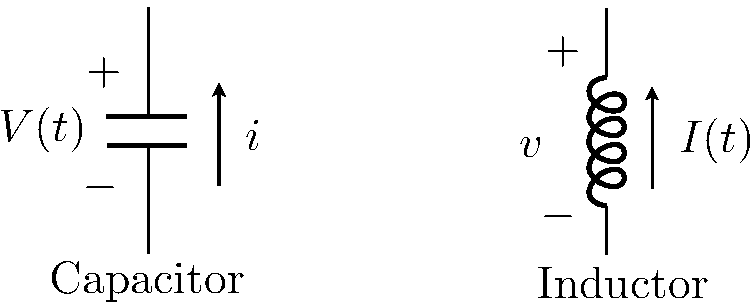
\includegraphics[height=1.5in]{5_fig_LC}}
\caption{Diagrams of capacitors and inductors. 
\label{fig_LC}}
\end{figure}

The voltage across the capacitor changes proportional to the current $i$ 
(with direction as in Figure~\ref{fig_LC}) through it 
\begin{equation}
\label{eq_cap}
\frac{dV}{dt} = - \frac{i}{C} 
\end{equation}
where the constant of proportionality $C$ is the capacitance of the capacitor
with MKS units of Farads. Note that a capacitor with large capacitance can 
provide more current for the same drop in voltage. 

The current through an inductor changes proportional to the voltage 
$v$ across it (with direction as in Figure~\ref{fig_LC}) 
\begin{equation}
\label{eq_ind}
\frac{dI}{dt} = - \frac{v}{L}
\end{equation}
where the constant of proportionality $L$ is the inductance with MKS 
units of Henrys. 

We consider here at a high level how the behaviour in time of 
circuits with many capacitors, inductors and resistors. At a given 
instant in time, capacitors can be treated as a voltage sources and 
inductors as current sources. To determine how these sources change 
in time, the current through the capacitors (\ref{eq_cap}) and the 
voltage across the inductors (\ref{eq_ind}) is needed. However, 
determining these from the sources is the {\em fundamental circuit 
problem} considered in Section~\ref{sec:loop} and Section~\ref{sec:retres}.
Thus, a system of differential equations can be derived for circuit 
networks with capacitors and inductors by solving the fundamental 
problem for the circuit and scaling the result by the capacitance and 
inductance of the elements. Some specific examples are given below. 

\subsection{Differential equations for LCR circuits}

\begin{figure}
\centerline{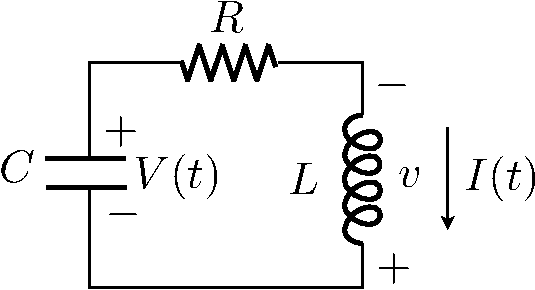
\includegraphics[height=1.5in]{5_fig_simpleLRC}}
\caption{A simple LRC circuit.
\label{fig_simpleLRC}}
\end{figure}

\begin{example} The simplest example of an LRC circuit is the 
simple series circuit shown in Figure~\ref{fig_simpleLRC}. We will 
derive a system of differential equations for $V(t)$ and $I(t)$ in 
the circuit and determine what combination of values for the 
components $L$, $R$, and $C$ lead to oscillations. 
{\rm The equation is simple enough that the solution to the 
fundamental problem can just be written down. The current through the 
capacitor is $I$ and the voltage $v$ across the inductor is $IR-V$. 
Using the relationships (\ref{eq_cap}, \ref{eq_ind}) we write 
\begin{eqnarray*}
\frac{dV}{dt} & = & - I/C \\
\frac{dI}{dt} & = & -(IR-V)/L = V/L - IR/L 
\end{eqnarray*}
or in matrix vector form 
\[
\xx^\prime = A \xx
\]
where $\xx = (V,I)^T$ and 
\[
A = \left[ \matrix{0 & -1/C \cr 1/L & -R/L} \right]
\]
The eigenvalues $\lambda$ of $A$ satisfy 
\[
\det (A-\lambda I) = \lambda^2 + \frac{R}{L} \lambda + \frac{1}{LC} = 0 
\]
with solutions 
\[
\lambda = \frac{1}{2L} \left(-R\pm \sqrt{R^2 - 4L/C} \right).
\]
Considering this expression carefully you can see that if the $\lambda$ 
values are real they are negative. If they are complex, the real part is 
$-R/(2L)$. Thus solutions always decay exponentially. This is to be 
expected in a circuit with no external power. For the circuit to have 
oscillations, the eigenvalues must be complex, so 
\[
R^2 - 4L/C < 0 
\]
which is commonly rewritten as 
\[
\frac{R}{2} \sqrt{\frac{C}{L}} < 1.
\]
}
\end{example}

\begin{figure}
\centerline{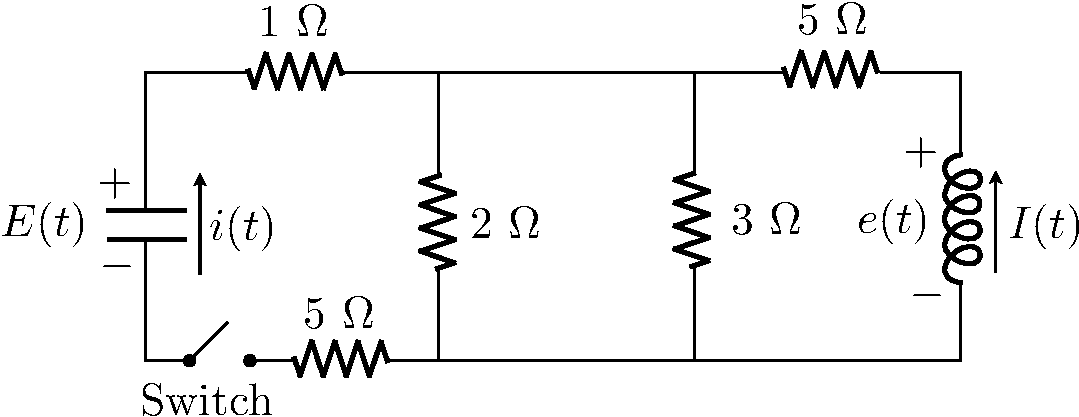
\includegraphics[height=1.5in]{5_fig_final}}
\caption{Circuit diagram for Example~\ref{ex_final}.
\label{fig_final}}
\end{figure}

\begin{example}
\label{ex_final} Consider the circuit shown in Figure~\ref{fig_final}. 
The capacitor has capacitance $C=1$ Farad and the inductor inductance 
$L=1$ Henry. The capacitor is charged up to 12V and then the switch is 
closed (so $E(0)=12$ and $I(0)=0$). 
\begin{enumerate}[(a)]
\item Derive a system of differential equations for $I(t)$ and $E(t)$.
\item We expect that $E(t)$ and $I(t) \rightarrow 0$ as $t \rightarrow 
\infty$ (no external power). Will there be oscillations in $E$ and $I$ 
in time? 
\end{enumerate} 
{\rm Remember that if $i(t)$ is the current upward through the capacitor 
then 
\begin{equation}
\label{eq_final1}
\frac{dE}{dt} = - \frac{i}{C} = - i 
\end{equation}
since $C=1$. If $e(t)$ is the voltage across the inductor as shown 
then 
\begin{equation}
\label{eq_final2}
\frac{dI}{dt} = - \frac{e}{L} = -e 
\end{equation}
since $L=1$. It is still necessary to work out $i(t)$ and $e(t)$ in 
terms of $E(t)$ and $I(t)$. This is the fundamental problem for the 
circuit. We solved this problem in Example 3.13 in Section 3.6 and 
considered it from a different perspective in the additional notes 
to Chapter 4. We found that 
\begin{eqnarray*}
i & = & \frac{5}{36} E - \frac{1}{6} I \\
e & = & \frac{1}{6} E + 6 I 
\end{eqnarray*}
Inserting these into (\ref{eq_final1}) and (\ref{eq_final2}) gives the 
desired system for $E$ and $I$:
\begin{eqnarray*}
\frac{dE}{dt} & = & -\frac{5}{36} E + \frac{1}{6} I \\
\frac{dI}{dt} & = & -\frac{1}{6} E - 6 I 
\end{eqnarray*}
or in vector form $\xx^\prime = A \xx$ where 
\[
\xx = \left[ \matrix{E \cr I} \right] \mbox{\ \ and \ \ }
A = \left[ \matrix{ -5/36 & 1/6 \cr -1/6 & - 6} \right]
\]
An eigenanalysis of $A$ gives $\lambda_1 \approx -0.1436$ and 
$\lambda_2 \approx -5.9953$. Since these are not complex, 
the circuit does not exhibit oscillations.
}
\end{example}

\subsection{Alternate description of LCR circuits} 

LCR circuits were presented differently in a previous version of the
notes. That approach is reproduced below starting in the next
paragraph. It follows the discussion in Section~\ref{sub_alternate}.

\begin{figure}
\centerline{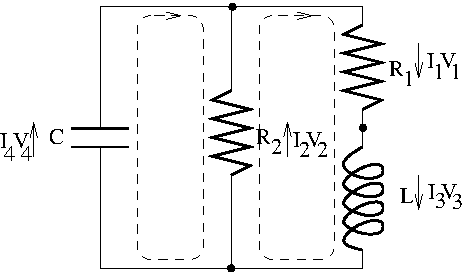
\includegraphics[height=1.5in]{5_circuit}}
\caption{Circuit diagram. 
\label{fig_circuit1}}
\end{figure}

We now return to the circuit that we discussed previously, shown in
Figure~\ref{fig_circuit1}.  Recall that we chose as basic variables
$I_3$ and $V_4$ and solved for all the other variables in terms of
these. The result was
\begin{eqnarray*}
I_1&=&I_3 \\
I_2&=&{{1}\over{R_2}}V_4 \\
I_4&=&I_3-{{1}\over{R_2}}V_4 \\
V_1&=&R_1I_3 \\
V_2&=&V_4 \\
V_3&=&-R_1I_3-V_4
\end{eqnarray*}
Now we can complete the job and determine $I_3$ and $V_4$. We have to
take into account now that the currents and voltages are functions of
time. The relations between currents and voltages across capacitors
and inductors involves the time derivatives.

If $I$ and $V$ are the current flowing through  and the voltage across
a capacitor with capacitance $C$, then
\[
{{dV}\over{dt}} = {{1}\over{C}}I
\]
If $I$ and $V$ are the current flowing through  and the voltage across
an inductor with inductance $L$, then
\[
{{dI}\over{dt}} = {{1}\over{L}}V
\]
Notice that we have chosen as basic the variables that get
differentiated.

Using these relations for $I_3$ and $V_4$ yields
\begin{eqnarray*}
{{dI_3}\over{dt}} &=& {{1}\over{L}}V_3 \\
{{dV_4}\over{dt}} &=& {{1}\over{C}}I_4
\end{eqnarray*}
Now we re-express everything in terms of $I_3$ and $V_4$ using the
equations we derived previously.
\begin{eqnarray*}
{{dI_3}\over{dt}} &=& {{1}\over{L}}(-R_1I_3-V_4)
={{-R_1}\over{L}}I_3 -{{1}\over{L}}V_4 \\
{{dV_4}\over{dt}} &=& {{1}\over{C}}(I_3-{{1}\over{R_2}}V_4)
={{1}\over{C}}I_3 -{{1}\over{R_2C}}V_4
\end{eqnarray*}
This can be written as 
\[
\left[\matrix{I_3\cr V_4\cr}\right]'
=\left[\matrix{{{-R_1}\over{L}}&-{{1}\over{L}}\cr
{{1}\over{C}}&-{{1}\over{R_2C}}\cr}\right]
\left[\matrix{I_3\cr V_4\cr}\right]
\]
Lets try to determine for what values of $R_1$, $L$, $C$ and $R_2$ the
circuit exhibits oscillations. Recall that the solution will involve
sines and cosines whenever the matrix has complex eigenvalues.

The polynomial $\det(A-\lambda I) = \lambda^2 + b\lambda + c$, where
\[
b={{R_1}\over{L}} + {{1}\over{R_2C}}
\]
and
\[
c= {{R_1}\over{R_2LC}} + {{1}\over{LC}}.
\]
The eigenvalues are the roots of this polynomial, given by
$(-b\pm\sqrt{b^2-4c})/2$. These will be complex if $b^2 < 4c$, i.e.,
if
\[
\left({{R_1}\over{L}} + {{1}\over{R_2C}} \right)^2 <
4\left({{R_1}\over{R_2LC}} + {{1}\over{LC}}\right)
\]
Notice that this can be achieved by decreasing $R_1$ and increasing $R_2$

\subsection{Problems}

\begin{problem} 
\label{op4_12}
In the circuit in Figure~\ref{fig_circuit1}, suppose that
$R_1=R_2=1$ ohm, $C=1$ farad and $L=1$ henry. If the initial current
across the inductor is $I_3(0)=1$ ampere and initial voltage across
the capacitor is $V_4(0) = 1$ volt, find $I_3(t)$ and $V_4(t)$ for all
later times. What is $V_1(t)$?  
\end{problem} 

\begin{figure}
\centerline{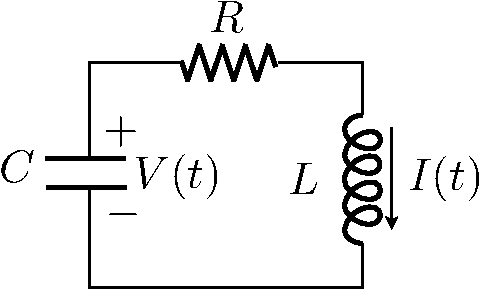
\includegraphics[height=1.5in]{5_circuit3}}
\caption{Circuit diagram for Problem~\ref{op4_13}. 
\label{fig_circuit3}}
\end{figure}

\begin{problem} 
\label{op4_13} Consider the
circuit with diagram in Figure~\ref{fig_circuit3}
Write down the system of equations satisfied by $I$ and $V$. For what values
of $L$, $C$ and $R$ does the circuit exhibit oscillations? Suppose that 
$R=1$ ohm, $C=1$ farad and $L=1$ henry. If the initial current across the
inductor is
$I(0)=1$ ampere and initial voltage across the capacitor is
$V(0) = 1$ volt, find $I(t)$ and $V(t)$ for all later times.
\end{problem}

\section{Additional Topics}

\subsection{Diagonalization}
\label{s_diagonalization}

Diagonal matrices (that is, matrices that have zero entries except on
the diagonal) are extremely easy to work with. For a start, the
eigenvalues of a diagonal matrix are exactly the diagonal entries. If
\[
D= \left[\matrix{\lambda_1&0&\cdots&0\cr 
		0&\lambda_2&\cdots&0\cr 
		\vdots&\vdots&&\vdots\cr
		0&0&\cdots&\lambda_n\cr}\right]
\]
then $\det(D-\lambda I) = (\lambda_1-\lambda)
(\lambda_2-\lambda)\cdots(\lambda_n-\lambda)$ which is zero precisely
when $\lambda$ equals one of $\lambda_1$, $\lambda_2$, $\ldots$,
$\lambda_n$. The corresponding eigenvectors are just the standard
basis vectors $\eee_1$, $\eee_2$, $\ldots$, $\eee_n$.

It is also easy to compute powers of a diagonal matrix. We simply obtain
\[
D^k = \left[\matrix{\lambda_1^k&0&\cdots&0\cr 
		0&\lambda_2^k&\cdots&0\cr 
		\vdots&\vdots&&\vdots\cr
		0&0&\cdots&\lambda_n^k\cr}\right]
\]
This formula makes it easy to compute the matrix exponential of
$D$. Recall that the matrix $e^{tD}$ is defined to be the matrix power
series
\[
e^{tD} = I + tD + {{t^2}\over{2}}D^2 + {{t^3}\over{3!}}D^3 + \cdots
\]
Using the formula above we find that
\begin{eqnarray*}
e^{tD} &= &
\left[\matrix{1&0&\cdots&0\cr 
		0&1&\cdots&0\cr 
		\vdots&\vdots&&\vdots\cr
		0&0&\cdots&1\cr}\right]
+
\left[\matrix{t\lambda_1&0&\cdots&0\cr 
		0&t\lambda_2&\cdots&0\cr 
		\vdots&\vdots&&\vdots\cr
		0&0&\cdots&t\lambda_n\cr}\right]
+
\left[\matrix{{{t^2\lambda_1^2}\over{2}}&0&\cdots&0\cr 
		0&{{t^2\lambda_2^2}\over{2}}&\cdots&0\cr 
		\vdots&\vdots&&\vdots\cr
		0&0&\cdots&{{t^2\lambda_n^2}\over{2}}\cr}\right]+\cdots \\
&=&\left[\matrix{1+t\lambda_1+{{t^2\lambda_1^2}\over{2}}+\cdots&0&\cdots&0\cr 
		0&1+t\lambda_2+{{t^2\lambda_2^2}\over{2}}&\cdots&0\cr 
		\vdots&\vdots&&\vdots\cr
		0&0&\cdots&1+t\lambda_n+{{t^2\lambda_n^2}\over{2}}+\cdots\cr}\right] \\
&=&\left[\matrix{e^{t\lambda_1}&0&\cdots&0\cr 
		0&e^{t\lambda_2}&\cdots&0\cr 
		\vdots&\vdots&&\vdots\cr
		0&0&e^{t\lambda_n}\cr}\right]
\end{eqnarray*}
Things are not quite so simple for an arbitrary $n\times n$ matrix
$A$. However, {\em if $A$ has a basis of eigenvectors} then it turns
out that there exists an invertible matrix $B$ such that $AB=DB$,
where $D$ is the diagonal matrix whose diagonal elements are the
eigenvalues of $A$. Multiplying by $B^{-1}$ from either the left or
right gives
\[
A=BDB^{-1}, \quad D=B^{-1}AB
\]
In fact, $B$ is simply the matrix whose columns are the eigenvectors
of $A$.  In other words, if $\xx_1$, $\xx_2$, $\ldots$, $\xx_n$ are
the eigenvectors for $A$ then $B=\left[\xx_1 \Big| \xx_2 \Big| \cdots
\Big| \xx_n \right]$.  To see this notice that
\begin{eqnarray*}
AB &=& A\left[\xx_1 \Big|  \xx_2 \Big| \cdots  \Big| \xx_n \right] \\
&=&\left[A\xx_1 \Big|  A\xx_2 \Big| \cdots  \Big| A\xx_n \right] \\
&=&\left[\lambda_1\xx_1 \Big|  \lambda_2\xx_2 \Big| \cdots  \Big|
   \lambda_n\xx_n \right] \\
&=&\left[\xx_1 \Big|  \xx_2 \Big| \cdots  \Big| \xx_n \right]
\left[\matrix{\lambda_1&0&\cdots&0\cr 
		0&\lambda_2&\cdots&0\cr 
		\vdots&\vdots&&\vdots\cr
		0&0&\cdots&\lambda_n\cr}\right] \\
&=& BD
\end{eqnarray*}
The assumption that $A$ has a basis of eigenvectors implies that the
matrix $B$ is invertible.

Using the representation $A=BDB^{-1}$ it is easy to calculate powers
of $A$.  We have
\[
A^2 = BDB^{-1}BDB^{-1} = BDIDB^{-1} = BD^2B^{-1}
\]
and similarly
\[
A^k = BD^kB^{-1}
\]
Therefore we can now also sum the power series for the exponential and obtain
\[
e^{tA} = Be^{tD}B^{-1}
\]

\subsection{Computing high powers of a matrix}
\label{s_powers}

Recall that when we were discussing the random walk problem, we ended
up with the problem of computing the limit for large $n$ of $P^n\xx_0$
where $P$ is the matrix of transition probabilities.

We can now solve this problem using diagonalization. Lets do an example.
Suppose that 
\[
P = \left[\matrix{{{1}\over{3}}&{{1}\over{4}}\cr
{{2}\over{3}}&{{3}\over{4}}\cr
}\right]
\]
We wish to compute $P^n$ for large $n$.

We begin by diagonalizing $P$. This involves finding the eigenvalues
and eigenvectors. I won't give the details of this computation. The
results are $\lambda_1=1$, $\xx_1=\left[\matrix{1\cr 8/3\cr}\right]$
and $\lambda_2=1/12$, $\xx_1=\left[\matrix{-1\cr 1\cr}\right]$. So
\[
P= \left[\matrix{1&-1\cr {{8}\over{3}}&1\cr}\right]
\left[\matrix{1&0\cr 0&{{1}\over{12}}\cr}\right]
\left[\matrix{1&-1\cr {{8}\over{3}}&1\cr}\right]^{-1}
\]
and
\[
P^n = \left[\matrix{1&-1\cr {{8}\over{3}}&1\cr}\right]
\left[\matrix{1^n&0\cr 0&\left({{1}\over{12}}\right)^n\cr}\right]
\left[\matrix{1&-1\cr {{8}\over{3}}&1\cr}\right]^{-1}
\]
But $1^n=1$ for all $n$ and $\left({{1}\over{12}}\right)^n\rarr 0$ as
$n\rarr\infty$, since ${{1}\over{12}}<1$. So
\begin{eqnarray*}
\lim_{n\rarr \infty} P^n &=& \left[\matrix{1&-1\cr {{8}\over{3}}&1\cr}\right]
\left[\matrix{1&0\cr 0&0\cr}\right]
\left[\matrix{1&-1\cr {{8}\over{3}}&1\cr}\right]^{-1} \\
&=&\left[\matrix{1&-1\cr {{8}\over{3}}&1\cr}\right]
\left[\matrix{1&0\cr 0&0\cr}\right]
\left[\matrix{{{3}\over{11}}&{{3}\over{11}}\cr
   {{-8}\over{11}}&{{3}\over{11}}\cr}\right] \\
&=&\left[\matrix{{{3}\over{11}}&{{3}\over{11}}\cr
   {{8}\over{11}}&{{8}\over{11}}\cr}\right] 
\end{eqnarray*}

\subsection{Another formula for the determinant}

If $A$ has a basis of eigenvectors, then we can get another formula
for the determinant. Using the multiplicative property of the
determinant, we have
\[
\det(A) = \det(BDB^{-1}) = \det(B)\det(D)\det(B)^{-1}=\det(D).
\]
But $\det(D)$ is just the product of the diagonal elements, i.e., the 
eigenvalues. Thus the determinant of $A$ is the product of its eigenvalues:
\[
\det(A) = \lambda_1\lambda_2\cdots\lambda_n.
\]
Actually, this is true even if $A$ doesn't have a basis of
eigenvectors and isn't diagonalizable.

\subsection{The matrix exponential and differential equations}

The matrix exponential $e^{tA}$ can be used to solve the differential
equation
\[
\yy'(t) = A\yy(t)
\]
with initial condition 
\[
\yy(0) = \xx_0
\]
To see this notice that $e^{tA}$ satisfies the differential equation
${{d}\over{dt}}e^{tA} = Ae^{tA}$. This follows from the power series
representation
\[
e^{tA}=I + tA + {{t^2}\over{2}}A^2 + {{t^3}\over{3!}}A^3 + \cdots
\]
since
\begin{eqnarray*}
{{d}\over{dt}}e^{tA} &=& A + {{2t}\over{2}}A^2 + {{3t^2}\over{3!}}A^3
   + \cdots \\
&=&A + tA^2 + {{t^2}\over{2!}}A^3 + \cdots \\
&=&A(I + tA + {{t^2}\over{2}}A^2 +\cdots) \\
&=&Ae^{tA}
\end{eqnarray*}
Also
\[
e^{0A} = I
\]
These two facts imply that $\yy(t)=e^{tA}\xx_0$ is the solution to our
differential equation and initial condition, since $\yy'(t) =
{{d}\over{dt}}e^{tA}\xx_0 = Ae^{tA}\xx_0 = A\yy(t)$ and $\yy(0) =
e^{0A}\xx_0 = I\xx_0 = \xx_0$.

The matrix exponential is a nice theoretical construction.  However,
to actually compute the matrix exponential using diagonalization
involves just the same ingredients---computing the eigenvalues and
vectors---as our original solution. In fact it is more work.

However, there is one situation where the matrix exponential gives us
something new. This is the situation where $A$ does not have a basis
of eigenvectors.  The power series definition of the matrix
exponential still makes sense, and can compute it in certain special
cases. Consider the matrix $A=\left[\matrix{1&1\cr0&1}\right]$. This
matrix does not have a basis of eigenvectors. So it cannot be
diagonalized.  However, in a homework problem, you showed that $e^{tA}
= \left[\matrix{e^t&te^t\cr 0&e^t}\right]$. Thus the solution to
\[
\yy'(t) = \left[\matrix{1&1\cr 0&1}\right]\yy(t)
\]
with initial condition
\[
\yy(0) = \left[\matrix{2\cr 1\cr}\right]
\]
is
\[
\yy(t) = e^{tA}\left[\matrix{2\cr 1\cr}\right]
=\left[\matrix{e^t&te^t\cr 0&e^t}\right]\left[\matrix{2\cr 1\cr}\right]
=\left[\matrix{2e^t+te^t\cr e^t\cr}\right]
\]
Notice that this solution involves a power of $t$ in addition to
exponentials.

\subsection{Converting higher order equations into first order systems}

So far we have only considered first order differential equations. In
other words, the equations have only involved first derivatives
$y'(t)$ and not higher derivatives like $y''(t)$. However higher order
equations, especially second order equations, occur often in practical
problems. In this section we will show that a higher order linear
differential equation can be converted into an equivalent first order
system.

Suppose we want to solve the equation
\[
y''(t) + ay'(t) + by(t) = 0
\]
with initial conditions
\begin{eqnarray*}
y(0)&=&y_0 \\
y'(0)&=&y'_0
\end{eqnarray*}
Define the new functions $z_1(t)$ and $z_2(t)$ by
\begin{eqnarray*}
z_1(t) &=& y(t) \\
z_2(t) &=& y'(t) 
\end{eqnarray*}
Then
\[
\matrix{
z'_1(t) &= y'(t) &= z_2(t)&\cr
z'_2(t) &= y''(t) &= -ay'(t)-by(t) &= -az_2(t)-bz_1(t)\cr
}
\]
and
\begin{eqnarray*}
z_1(0) &=& y_0 \\
z_2(0) &=& y'_0 \\
\end{eqnarray*}

In other words the vector $\left[\matrix{z_1(t)\cr z_2(t)\cr}\right]$
satisfies the equation
\[
{{d}\over{dt}}\left[\matrix{z_1(t)\cr z_2(t)\cr}\right]
=\left[\matrix{0 &1 \cr -b& -a \cr}\right]
\left[\matrix{z_1(t)\cr z_2(t)\cr}\right]
\]
with initial condition
\[
\left[\matrix{z_1(0)\cr z_2(0)\cr}\right] =
\left[\matrix{y_0\cr y'_0\cr}\right]. 
\]

\begin{example}
Suppose we want to solve the second order equation
\[
y'' + 4y' + y = 0
\]
with initial conditions
\[
y(0)=1, y'(0)=0
\]
{\rm If we let $z_1(t) = y(t)$ and $z_2(t)  = y'(t)$ then
\[
{{d}\over{dt}}\left[\matrix{z_1(t)\cr z_2(t)\cr}\right]
=\left[\matrix{0 &1 \cr -1& -4 \cr}\right]
\left[\matrix{z_1(t)\cr z_2(t)\cr}\right]
\]
with initial condition
\[
\left[\matrix{z_1(0)\cr z_2(0)\cr}\right] =
\left[\matrix{1\cr 0\cr}\right]. 
\]
To solve this we first find the eigenvalues and eigenvectors. They
are $\lambda_1=-2+\sqrt{3}$, $\xx_1=\left[\matrix{1\cr-2+\sqrt{3}\cr}\right]$
and $\lambda_1=-2-\sqrt{3}$, $\xx_1=\left[\matrix{1\cr-2-\sqrt{3}\cr}\right]$
So the general solution is 
\[
c_1e^{(-2+\sqrt{3})t}\left[\matrix{1\cr-2+\sqrt{3}\cr}\right]
+c_2e^{(-2-\sqrt{3})t}\left[\matrix{1\cr-2-\sqrt{3}\cr}\right]
\]
To satisfy the initial condition, we need
\[
c_1 \left[\matrix{1\cr-2+\sqrt{3}\cr}\right] +
c_2 \left[\matrix{1\cr-2-\sqrt{3}\cr}\right] = 
\left[\matrix{1\cr 0\cr}\right]
\]
The solution is
\[
\left[\matrix{c_1\cr c_2\cr}\right] = 
\left[\matrix{\sqrt{3}/3 + 1/2\cr -\sqrt{3}/3 + 1/2\cr}\right]
\]
Thus
\[
\left[\matrix{z_1(t)\cr z_2(t)\cr}\right]=
(\sqrt{3}/3 + 1/2)e^{(-2+\sqrt{3})t}\left[\matrix{1\cr-2+\sqrt{3}\cr}\right]
+(-\sqrt{3}/3 + 1/2)e^{(-2-\sqrt{3})t}\left[\matrix{1\cr-2-\sqrt{3}\cr}\right]
\]
and so
\[
y(t)=z_1(t) = (\sqrt{3}/3 + 1/2)e^{(-2+\sqrt{3})t} + 
(-\sqrt{3}/3 + 1/2)e^{(-2-\sqrt{3})t}
\]}
\end{example}

Actually, to solve the equation
\[
y''(t) + ay'(t) + by(t) = 0
\]
it is not really necessary to turn it into a first order system. We
can simply try to find solutions of the form $y(t)=e^{\lambda t}$. If
we plug this into the equation we get $(\lambda^2 + a\lambda +
b)e^{\lambda t}$ which is zero if $\lambda$ is a root of $\lambda^2 +
a\lambda + b$. This polynomial has two roots, which yields two
solutions.

Still, the procedure of turning a higher order equation into a first
order system is important. This is because on a computer it is much
easier to solve a first order system than a high order equation. If
the coefficients $a$ and $b$ are functions of $t$, then exact
solutions (like exponentials) usually can't be found. However, one can
still turn the equation into a first order system $\yy'(t) =
A(t)\yy(t)$ where the matrix now depends on $t$ and solve this on a
computer.

\subsection{Springs and weights}

To begin, lets consider the situation where we have a single weight
hanging on a spring shown in Figure~\ref{fig_spring}.  We want to
determine how the weight moves in time. To do this we calculate the
forces acting on the weight and use Newton's law of motion $F=ma$.

\begin{figure}
\centerline{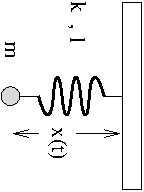
\includegraphics[height=1.5in]{5_spring}}
\caption{A simple mass-spring system.
\label{fig_spring}}
\end{figure}

One force acting on the weight are the force of gravity. This acts in
the positive $x$ direction (i.e., downward) and has magnitude
$mg$. The other force is due to the spring. It's magnitude is $k(x-l)$
in the negative $x$ direction. The acceleration is the second
derivative $x''(t)$. Thus the total force is $F = mg - k(x(t)-l)$ and
$ma=mx''(t)$ Newton's law reads
\[
mx''(t) = mg - k(x-l) = -kx + mg + lk
\]

This is not quite in the form we can handle, due to the term $mg+lk$
on the right. What we must do is first find the equilibrium
solution. In a previous lecture we found the equilibrium position by
minimizing the potential energy.  There is another, equivalent,
way. That is to find the value of $x$ for which the total force is
zero. In other words
\[
-kx_{\rm eq} + mg + lk = 0
\]
or 
\[
x_{\rm eq} = (mg + lk)/k
\]
Notice that the total force can be written
\[
-kx + mg + lk = -k(x-x_{\rm eq})
\]
Now let $y(t)=x(t)-x_{\rm eq}$ be the displacement from the
equilibrium point.  Notice that $y'(t)=x'(t)$ and $y''(t) = x''(t)$,
since $x_{\rm eq}$ is a constant.  So the equation for $y(t)$ is
\[
m y''(t) = -ky(t)
\]
or 
\[
y''(t) + {{k}\over{m}}y(t) = 0
\]

We could turn this into a first order system. However, it is easier to
try solutions of the form $e^{\lambda t}$. Substituting this into the
equation yields
\[
(\lambda^2 + k/m)e^{\lambda t}=0
\]
so we require that $\lambda^2 + k/m=0$, or $\lambda=\pm i\sqrt{k/m}$.
Thus, solutions are $e^{i\sqrt{k/m}t}$ and $e^{-i\sqrt{k/m}t}$. To
obtain real solutions, we can take the real and imaginary parts. This
gives as solutions $\sin(\sqrt{k/m} t)$ and $\cos(\sqrt{k/m} t)$ , and
the general solution is
\[
c_1\sin(\sqrt{k/m} t) + c_2\cos(\sqrt{k/m} t)
\]

We can make the equation a little more interesting by adding friction.
A frictional force is proportional to the velocity and acts in the
direction opposite to the motion. Thus the equation with friction
reads
\[
y''(t) + \beta y'(t) + {{k}\over{m}}y(t) = 0
\]
This can be solved by turning it into a first order system, or
directly, using trial solution of the form $e^{\lambda t}$ as above.

Now we turn the problem with several weights and springs shown in
Figure~\ref{fig_springs1}. In this problem matrices play an essential
role.

\begin{figure}
\centerline{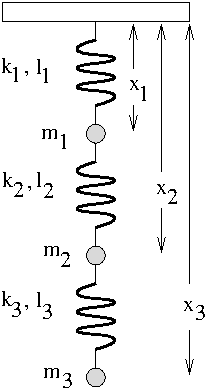
\includegraphics[height=1.5in]{5_springs}}
\caption{A more complicated mass-spring system.
\label{fig_springs1}}
\end{figure}

We begin by computing the forces acting on each weight.  Let us start
with the first weight. Gravity is pulling down, and the springs above
and below are pushing or pulling with a force proportional to their
extensions. Thus the total force on the first weight is $m_1g -
k_1(x_1-l_1) + k_2(x_2-x_1-l_2)$. To get the signs right on the spring
forces, think of what happens when one of the $x_i$'s gets large. For
example, when $x_1$ gets large, the first spring stretches and pulls
up, so the sign of the force should be negative for large $x_1$. So
Newton's equation for the first weight is
\[
m_1 x_1''(t) = m_1g - k_1(x_1-l_1) + k_2(x_2-x_1-l_2)
=-(k_1+k_2)x_1 + k_2x_2 + m_1g + k_1l_1 - k_2l_2
\]
or
\[
x_1''(t) =-{{k_1+k_2}\over{m_1}}x_1 + {{k_2}\over{m_1}}x_2 + g 
+ {{k_1l_1 - k_2l_2}\over{m_1}}
\]
Similarly the equations for the second and third weights are
\begin{eqnarray*}
x_2''(t) &=& {{k_2}\over{m_2}}x_1 - {{k_2+k_3}\over{m_2}}x_2
   +{{k_3}\over{m_2}}x_3 +g + {{k_2l_2-k_3l_3}\over{m_2}} \\
x_3''(t) &= &{{k_3}\over{m_3}}x_2 -{{k_3}\over{m_3}}x_3 + g
   +{{k_3l_3}\over{m_3}} \\
\end{eqnarray*}
Thus can be written as a second order matrix equation
\[
\xx''(t) = K\xx(t) + \bb
\]
where
\[
\xx(t) = \left[\matrix{x_1(t)\cr x_2(t)\cr x_3(t)\cr}\right],
\] 
\[
K=\left[\matrix{-{{k_1+k_2}\over{m_1}}&{{k_2}\over{m_1}}&0\cr
{{k_2}\over{m_2}}&- {{k_2+k_3}\over{m_2}}&{{k_3}\over{m_2}}\cr
0&{{k_3}\over{m_3}}&-{{k_3}\over{m_3}}\cr}\right]
\]
and 
\[
\bb = \left[\matrix{
g + {{k_1l_1 - k_2l_2}\over{m_1}}\cr
g + {{k_2l_2 - k_3l_3}\over{m_2}}\cr
g + {{k_3l_3}\over{m_3}}\cr
}\right].
\]
With this notation, the equilibrium solution is the value of $\xx$
that makes all the forces zero. That is,
\[
K\xx_{\rm eq} + \bb = \zv
\]
or,
\[
\xx_{\rm eq} = -K^{-1}\bb
\]
As in the case of one weight the force side of the equation can now be
written as
\[
K\xx + b = K(\xx + K^{-1}\bb) = K(\xx-\xx_{\rm eq})
\]
so if we define
\[
\yy(t) = \xx(t) -\xx_{\rm eq},
\]
the equation for $\yy(t)$ is
\[
\yy''(t) = K\yy(t)
\]

To solve this second order $3\times 3$ system, we could turn it in to
a first order $6\times 6$ system. However, just as in the case of a
single higher order equation we can proceed directly. We try trial
solutions of the form $e^{\kappa t}\yy$. Substituting this into the
equation, we see that the equation is satisfied if
\[
\kappa^2\yy = K\yy
\]
in other words, $\kappa^2$ is an eigenvalue of $K$ with eigenvector
$\yy$, or $\kappa$ is one of the two square roots of and eigenvalue.

So, if $K$ has eigenvalues $\lambda_1$, $\lambda_2$ and $\lambda_3$
with eigenvectors $\yy_1$, $\yy_2$ and $\yy_3$, then six solutions of
the equation are given by $e^{\sqrt{\lambda_1}t}\yy_1$,
$e^{-\sqrt{\lambda_1}t}\yy_1$, $e^{\sqrt{\lambda_2}t}\yy_2$,
$e^{-\sqrt{\lambda_2}t}\yy_2$, $e^{\sqrt{\lambda_3}t}\yy_3$ and
$e^{-\sqrt{\lambda_3}t}\yy_3$.  If some of the $\lambda_i$'s are
negative, then these solutions are complex exponentials, and we may
take their real and imaginary parts to get real solutions. The general
solution is a linear combination of these, and the coefficients in the
linear combination may be chosen to satisfy an initial condition.

To make this clear we will do an example. Suppose that all the masses
$m_i$, lengths $l_i$ and spring constants $k_i$ are equal to $1$. Then
\[
K=\left[\matrix{-2&1&0\cr 1&-2&1\cr 0&1&-1\cr}\right]
\]
Suppose that the initial position of the weights is $x_1 = 30$, $x_2=60$
and $x_3=70$, and that the initial velocities are $x_1'=1$ and $x_2' =
x_3' = 0$. We will determine the positions of the weights for all
subsequent times. The numbers in this problem don't turn out
particularly nicely, so I'll just give them to 3 significant figures.

The first step is to find the eigenvalues and eigenvectors of
$K$. They are given by
\[
\lambda_1 = -0.198 \quad \lambda_2 = -1.55 \quad \lambda_3 = -3.25
\]
\[
\xx_1 = \left[\matrix{0.445\cr 0.802\cr 1.00\cr}\right] \quad
\xx_2 = \left[\matrix{-1.25\cr -0.555\cr 1.00\cr}\right] \quad
\xx_3 = \left[\matrix{1.80\cr -2.25\cr 1.00\cr}\right]
\]
Let $\mu_1=\sqrt{0.198}=0.445$, $\mu_2=\sqrt{1.55}=1.25$ and
$\mu_3=\sqrt{3.25}=1.80$ Then if $\yy(t)=\xx(t)-\xx_{\rm eq}$, then
general solution for $\yy(t)$ is
\[
\yy(t) = (c_1 e^{i\mu_1t} + d_1 e^{-i\mu_1t})\xx_1 +
         (c_2 e^{i\mu_2t} + d_2 e^{-i\mu_2t})\xx_2 +
         (c_3 e^{i\mu_3t} + d_3 e^{-i\mu_3t})\xx_3
\]
where $c_1, d_1, c_2, d_2 , c_3, d_3$ are arbitrary constants. Taking real
and imaginary parts, we can also write the general solution as
\[
\yy(t) = (a_1 \cos({\mu_1t}) + b_1 \sin({\mu_1t}))\xx_1 +
         (a_2 \cos({\mu_2t}) + b_2 \sin({\mu_2t}))\xx_2 +
         (a_3 \cos({\mu_3t}) + b_3 \sin({\mu_3t}))\xx_3
\]
where $a_1, b_1, a_2, b_2 , a_3, b_3$ are arbitrary constants.  Notice
that we can find the general solution for $\yy(t)=\xx(t)-\xx_{\rm eq}$
without knowing $\xx_{\rm eq}$. However, since the initial conditions
were given in terms of $\xx$ and not $\yy$, we now have to find
$\xx_{\rm eq}$ to be able to convert initial conditions for $\xx$ to
initial conditions for $\yy$.  If we work in units where $g=10$ then
\[
\bb=\left[\matrix{10\cr 10\cr 11\cr}\right]
\]
and
\[
\xx_{\rm eq} = -K^{-1}\bb = \left[\matrix{31\cr 52\cr 63\cr}\right]
\]
so
\[
\yy(0) = \xx(0)-\xx_{\rm eq} =
\left[\matrix{30\cr 60\cr 70\cr}\right]-\left[\matrix{31\cr 52\cr 63\cr}\right]
=\left[\matrix{-1\cr 8\cr 7\cr}\right]
\]
Also
\[
\yy'(0) = \xx'(0) = \left[\matrix{1\cr 0\cr 0\cr}\right]
\]
So to satisfy the first initial condition, since $\cos(0)=1$ and
$\sin(0)=0$, we need that
\[
\yy(0) = a_1 \xx_1 +
         a_2 \xx_2 +
         a_3 \xx_3 = \left[\matrix{-1\cr 8\cr 7\cr}\right].
\]
Explicitly, we need to solve
\[
\left[\xx_1 | \xx_2 | \xx_3 \right]\left[\matrix{a_1\cr a_2\cr a_3\cr}\right]
=\left[\matrix{-1\cr 8\cr 7\cr}\right],
\]
or
\[
\left[\matrix{0.445&-1.25&1.80\cr 0.802&-0.555&-2.25\cr
1.00&1.00&1.00\cr}\right] \left[\matrix{a_1\cr a_2\cr a_3\cr}\right]
=\left[\matrix{-1\cr 8\cr 7\cr}\right]
\]
This is not a pretty sight, but I can punch the numbers into my
computer and find that
\[
\left[\matrix{a_1\cr a_2\cr a_3\cr}\right]
=\left[\matrix{7.04\cr 1.33\cr -1.37\cr}\right]
\]
To satisfy the second initial condition, we differentiate the
expression for the general solution of $\yy(t)$ and set $t=0$. This
gives
\[
\mu_1b_1\xx_1 + \mu_2b_2\xx_2 + \mu_3b_3\xx_3
=\left[\matrix{1\cr 0\cr 0\cr}\right]
\]
Solving this numerically gives
\[
\left[\matrix{\mu_1b_1\cr \mu_2b_2\cr \mu_3b_3\cr}\right]
=
\left[\matrix{0.242\cr -0.435\cr 0.194\cr}\right]
\]
Finally, we divide by the $\mu_i's$ to give
\[
\left[\matrix{b_1\cr b_2\cr b_3\cr}\right]
=\left[\matrix{0.543\cr -0.348\cr 1.80\cr}\right]
\]
Now we have completely determined all the constants, so the solution
is complete.

\subsection{Problems}

\begin{problem}
\label{op4_14}
Consider the second order equation
\[
y'' - 5y' + 6y = 0
\]
with initial conditions $y(0)=1$, $y'(0)=0$. Solve this by turning it
into a $2\times 2$ system. Then solve it directly by using trial solutions
$e^{\lambda t}$.
\end{problem}

\begin{problem}
\label{op4_15}
Consider the second order equation
\[
y''+y' + y = 0
\]
with initial conditions $y(0)=1$, $y'(0)=0$. Solve this by turning it
into a $2\times 2$ system. Then solve it directly by using trial
solutions $e^{\lambda t}$.  
\end{problem}

\begin{problem}
\label{op4_16} 
How can you turn a third order equation
\[
y''' + a y'' + by' + cy=0
\]
into an equivalent $3\times 3$ system of equations?
\end{problem}

\begin{problem}
\label{op4_17}
Suppose $K$ is a $3 \times 3$ matrix with eigenvalues and eigenvectors
given by
\[
\lambda_1 = -1 \quad \lambda_2 = -4 \quad \lambda_3 = -9
\]
\[
\xx_1 = \left[\matrix{1\cr 0\cr 1\cr}\right] \quad
\xx_2 = \left[\matrix{1\cr 0\cr -1\cr}\right] \quad
\xx_3 = \left[\matrix{0\cr 1\cr 0\cr}\right]
\]
Find the solution of 
\[
\yy''(t) = K\yy(t)
\]
satisfying
\[
\yy(0) = \left[\matrix{1\cr 2\cr 1\cr}\right]
\]
\[
\yy'(0) = \left[\matrix{0\cr 1\cr 1\cr}\right]
\]
\end{problem}

\begin{problem}
\label{op4_18}
Consider a system of two hanging weights and springs. Suppose that all
the masses, spring constants and spring lengths are equal to one, and
that $g=10$. Find the positions $x_1(t)$ and $x_2(t)$ for all times if
$x_1(0)=20$, $x_2(0)=30$, $x'_1(0)=1$, $x'_2(0)=1$.
\end{problem}

\section{Solutions to Chapter Problems}

%%%%%%%%%%%%%%%%%%%%%%%%%%%%%%%%%%%%%%%%%%%%%%%%%%%%%%%%%%%%%%%%%%%%%%%%%%%%%%%%
\noindent {\bf Solution~\ref{op4_1}}
We compute $\left[\matrix{1&1\cr 1&1\cr}\right]\left[\matrix{1\cr 1\cr}\right]
=\left[\matrix{2\cr 2\cr}\right]=2\left[\matrix{1\cr 1\cr}\right]$,
so $\left[\matrix{1\cr 1\cr}\right]$ is an eigenvector with eigenvalue $2$.
Also $\left[\matrix{1&1\cr 1&1\cr}\right]\left[\matrix{1\cr -1\cr}\right]
=\left[\matrix{0\cr 0\cr}\right]=0\left[\matrix{1\cr -1\cr}\right]$,
so $\left[\matrix{1\cr -1\cr}\right]$ is an eigenvector with eigenvalue $0$.

%%%%%%%%%%%%%%%%%%%%%%%%%%%%%%%%%%%%%%%%%%%%%%%%%%%%%%%%%%%%%%%%%%%%%%%%%%%%%%%%
\vspace{2mm}
\noindent {\bf Solution~\ref{op4_2}}
If $P$ projects onto some line, then a vector $\xx$ lying on that line doesn't
get changed by $P$ so $P\xx = \xx$ and $\xx$ is an eigenvector with eigenvalue
$1$. On the other hand, if $\xx$ is perpendicular to the line, then
$P\xx=\zv=0\xx$
so $\xx$ is an eigenvector with eigenvalue $0$.

%%%%%%%%%%%%%%%%%%%%%%%%%%%%%%%%%%%%%%%%%%%%%%%%%%%%%%%%%%%%%%%%%%%%%%%%%%%%%%%%
\vspace{2mm}
\noindent {\bf Solution~\ref{op4_3}}
\begin{enumerate}[a)]
\item $\det(A-\lambda I) = \lambda^2-9 = (\lambda-3)(\lambda+3)$
so the eigenvalues are $\lambda_1=3$ and $\lambda_2=-3$.
To find the eigenvector for $\lambda_1=3$ we must solve the homogeneous equation
with matrix
$\left[\matrix{-3&3\cr 3&-3\cr}\right]$. The matrix reduces to
$\left[\matrix{-3&3\cr 0&0\cr}\right]$ and the eigenvector is
$\xx_1=\left[\matrix{1\cr 1\cr}\right]$.
To find the eigenvector for $\lambda_2=-3$ we must solve the homogeneous equation
with matrix
$\left[\matrix{3&3\cr 3&3\cr}\right]$. The matrix reduces to
$\left[\matrix{3&3\cr 0&0\cr}\right]$ and the eigenvector is
$\xx_2=\left[\matrix{1\cr -1\cr}\right]$.
\item $\det(A-\lambda I) = \lambda^2-8\lambda+12 = (\lambda-2)(\lambda-6)$
so the eigenvalues are $\lambda_1=3$ and $\lambda_2=-3$.
To find the eigenvector for $\lambda_1=2$ we must solve the homogeneous equation
with matrix
$\left[\matrix{-4&-8\cr 4&8\cr}\right]$. The matrix reduces to
$\left[\matrix{-4&-8\cr 0&0\cr}\right]$ and the eigenvector is
$\xx_1=\left[\matrix{2\cr -1\cr}\right]$.
To find the eigenvector for $\lambda_2=6$ we must solve the homogeneous equation
with matrix
$\left[\matrix{-8&-8\cr 4&4\cr}\right]$. The matrix reduces to
$\left[\matrix{-8&-8\cr 0&0\cr}\right]$ and the eigenvector is
$\xx_2=\left[\matrix{1\cr -1\cr}\right]$.
\item $\det(A-\lambda I) = \lambda^2+7\lambda+6 = (\lambda+6)(\lambda+1)$
so the eigenvalues are $\lambda_1=-6$ and $\lambda_2=-1$.
To find the eigenvector for $\lambda_1=-6$ we must solve the homogeneous equation
with matrix
$\left[\matrix{35&-10\cr 105&-30\cr}\right]$. The matrix reduces to
$\left[\matrix{35&-10\cr 0&0\cr}\right]$ and the eigenvector is
$\xx_1=\left[\matrix{2\cr 7\cr}\right]$.
To find the eigenvector for $\lambda_2=-1$ we must solve the homogeneous equation
with matrix
$\left[\matrix{30&-10\cr 105&-35\cr}\right]$. The matrix reduces to
$\left[\matrix{30&-10\cr 0&0\cr}\right]$ and the eigenvector is
$\xx_2=\left[\matrix{1\cr 3\cr}\right]$.
\item $\det(A-\lambda I) = \lambda^2-3\lambda-10 = (\lambda+2)(\lambda-5)$
so the eigenvalues are $\lambda_1=-2$ and $\lambda_2=5$.
To find the eigenvector for $\lambda_1=-2$ we must solve the homogeneous equation
with matrix
$\left[\matrix{-7&-14\cr 7&14\cr}\right]$. The matrix reduces to
$\left[\matrix{-7&-14\cr 0&0\cr}\right]$ and the eigenvector is
$\xx_1=\left[\matrix{2\cr -1\cr}\right]$.
To find the eigenvector for $\lambda_2=5$ we must solve the homogeneous equation
with matrix
$\left[\matrix{-14&-14\cr 7&7\cr}\right]$. The matrix reduces to
$\left[\matrix{-14&-14\cr 0&0\cr}\right]$ and the eigenvector is
$\xx_2=\left[\matrix{1\cr -1\cr}\right]$.
\end{enumerate}

%%%%%%%%%%%%%%%%%%%%%%%%%%%%%%%%%%%%%%%%%%%%%%%%%%%%%%%%%%%%%%%%%%%%%%%%%%%%%%%%
\vspace{2mm}
\noindent {\bf Solution \ref{2009_a10_4}}
\begin{eqnarray*}
  \det\left[\begin{array}{cc}2-\lambda&3\\2&1-\lambda\end{array}\right]&=&(2-\lambda)(1-\lambda)-6 = 2-3\lambda+\lambda^2-6\\
	&=& \lambda^2-3\lambda-4 = (\lambda-4)(\lambda-5)=0\\
	&\Rightarrow& \lambda = -1,4.
\end{eqnarray*}
The eigenvector for $\lambda=-1$:
$$
\left[\begin{array}{cc}3&3\\2&2\end{array}\right]\left[\begin{array}{c}k_1\\k_2\end{array}\right]=\vec{0}\qquad\Rightarrow\qquad
\begin{array}{c}3k_1+3k_2=0\\2k_1+2k_2=0\end{array}\qquad\Rightarrow\qquad k_1=-k_2
$$
If we set $k_2=1$ for convenience, we have that the first eigenpair is
$$
\lambda_1=-1,\qquad\vec{v}_1=\left[\begin{array}{c}-1\\1\end{array}\right].
$$
Now, the eigenvector for $\lambda=4$:
$$
\left[\begin{array}{cc}-2&3\\2&-3\end{array}\right]\left[\begin{array}{c}k_1\\k_2\end{array}\right]=\vec{0}\qquad\Rightarrow\qquad
\begin{array}{c}-2k_1+3k_2=0\\2k_1-3k_2=0\end{array}\qquad\Rightarrow\qquad k_1=\frac{3}{2} k_2
$$
If we set $k_2=1$ for convenience, we have that the second eigenpair is
$$
\lambda_2=4,\qquad\vec{v}_2=\left[\begin{array}{c}3/2\\1\end{array}\right].
$$
%%%%%%%%%%%%%%%%%%%%%%%%%%%%%%%%%%%%%%%%%%%%%%%%%%%%%%%%%%%%%%%%%%%%%%%%%%%%%%%%
\vspace{2mm}
\noindent {\bf Solution~\ref{op4_4}}
\begin{enumerate}[a)]
\item $\det(A-\lambda I) = -\lambda^3  +2\lambda^2  +\lambda  -2
= -(\lambda-1)(\lambda-2)(\lambda+1)$
so the eigenvalues are $\lambda_1=1$ and $\lambda_2=2$ and $\lambda_3=-1$.
To find the eigenvector for $\lambda_1=1$ we must solve the homogeneous equation
with matrix
$\left[\matrix{-1&-1&1\cr 1&-1&2\cr 2&0&1\cr}\right]$. The matrix reduces to
$\left[\matrix{-1&-1&1\cr 0&-2&3\cr 0&0&0\cr}\right]$ and the eigenvector is
$\xx_1=\left[\matrix{1\cr-3\cr 2\cr}\right]$.
To find the eigenvector for $\lambda_2=2$ we must solve the homogeneous equation
with matrix
$\left[\matrix{-2&-1&1\cr 1&-2&2\cr 2&0&0\cr}\right]$. The matrix reduces to
$\left[\matrix{-2&-1&1\cr 0&-1&1\cr 0&0&0\cr}\right]$ and the eigenvector is
$\xx_2=\left[\matrix{0\cr 1\cr 1}\right]$.
To find the eigenvector for $\lambda_3=-1$ we must solve the homogeneous equation
with matrix
$\left[\matrix{1&-1&1\cr 1&1&2\cr 2&0&3\cr}\right]$. The matrix reduces to
$\left[\matrix{1&-1&1\cr 0&2&1\cr 0&0&0\cr}\right]$ and the eigenvector is
$\xx_3=\left[\matrix{3\cr 1\cr -2}\right]$.
\item $\det(A-\lambda I) = -\lambda^3  +2\lambda^2  +3\lambda-6  =
-(\lambda-2)(\lambda-\sqrt{3})(\lambda+\sqrt{3})$
so the eigenvalues are $\lambda_1=2$ and $\lambda_2=\sqrt{3}$ and $\lambda_3=-\sqrt{3}$..
To find the eigenvector for $\lambda_1=2$ we must solve the homogeneous equation
with matrix
$\left[\matrix{-1&1&1\cr 1&-2&-2\cr 1&-1&-1\cr}\right]$. The matrix reduces to
$\left[\matrix{ 0&-1&-1\cr 0&0&0\cr-1&1&1\cr}\right]$ and the eigenvector is
$\xx_1=\left[\matrix{0\cr -1\cr 1\cr}\right]$.
To find the eigenvector for $\lambda_2=\sqrt{3}$ we must solve the homogeneous equation
with matrix
$\left[\matrix{1-\sqrt{3}&1&1\cr 1&-\sqrt{3}&-2\cr 1&-1&1-\sqrt{3}\cr}\right]$. 
The matrix reduces to
$\left[\matrix{1-\sqrt{3}&1&1\cr 0&2-\sqrt{3}&-3+2\sqrt{3}\cr0&0&0\cr}\right]$ and the eigenvector is
$\xx_2=\left[\matrix{-1\cr-\sqrt{3}\cr 1}\right]$.
To find the eigenvector for $\lambda_3=-\sqrt{3}$ we must solve the homogeneous equation
with matrix
$\left[\matrix{1+\sqrt{3}&1&1\cr 1&+\sqrt{3}&-2\cr 1&-1&1+\sqrt{3}\cr}\right]$. 
The matrix reduces to
$\left[\matrix{1+\sqrt{3}&1&1\cr 0& 2+\sqrt{3}&2\sqrt{3}+1\cr0&0&0\cr}\right]$ and the eigenvector is
$\xx_3=\left[\matrix{-1\cr \sqrt{3}\cr 1}\right]$.
\item $\det(A-\lambda I) = -\lambda^3  +48\lambda -128 = -(\lambda+8)(\lambda-4)^2$
so the eigenvalues are $\lambda_1=-8$ and $\lambda_2=4$.
To find the eigenvector for $\lambda_1=-8$ we must solve the homogeneous equation
with matrix
$\left[\matrix{15&-9&-15\cr 0&12&0\cr 3&-9&-3}\right]$. The matrix reduces to
$\left[\matrix{15&-9&-15\cr 0&12&0\cr 0&0&0}\right]$ and the eigenvector is
$\xx_1=\left[\matrix{1\cr 0\cr 1}\right]$.
To find the eigenvector(s) for $\lambda_2=4$ we must solve the homogeneous equation
with matrix
$\left[\matrix{3&-9&-15\cr 0&4&0\cr 3&-9&-15}\right]$. The matrix reduces to
$\left[\matrix{3&-9&-15\cr 0&0&0\cr 0&0&0\cr}\right]$. Thus there are two
eigenvectors corresponding to this eigenvalues, for example
$\xx_2=\left[\matrix{3\cr1\cr0}\right]$ and $\xx_3=\left[\matrix{5\cr0\cr1}\right]$.
\item $\det(A-\lambda I) = -\lambda^3  +\lambda^2  +\lambda -1 
= -(\lambda+1)(\lambda-1)^2$
so the eigenvalues are $\lambda_1=-1$ and $\lambda_2=1$.
To find the eigenvector for $\lambda_1=-1$ we must solve the homogeneous equation
with matrix
$\left[\matrix{32&-100&70\cr 18&-58&42\cr 12&-40&30}\right]$. The matrix reduces to
$\left[\matrix{32&-100&70\cr0&-14&21\cr0&0&0\cr}\right]$ and the eigenvector is
$\xx_1=\left[\matrix{5\cr3\cr 2}\right]$.
To find the eigenvector for $\lambda_2=1$ we must solve the homogeneous equation
with matrix
$\left[\matrix{30&-100&70\cr 18&-60&42\cr 12&-40&28}\right]$. The matrix reduces to
$\left[\matrix{30&-100&70\cr 0&0&0\cr0&0&0\cr}\right]$Thus there are two
eigenvectors corresponding to this eigenvalues, for example
$\xx_2=\left[\matrix{7\cr0\cr-3}\right]$ and $\xx_3=\left[\matrix{0\cr7\cr10}\right]$.
\end{enumerate}

%%%%%%%%%%%%%%%%%%%%%%%%%%%%%%%%%%%%%%%%%%%%%%%%%%%%%%%%%%%%%%%%%%%%%%%%%%%%%%%%
\vspace{2mm}
\noindent {\bf Solution \ref{2009_a10_5}}
\begin{eqnarray*}
  \det\left[\begin{array}{cc}p_{11}-\lambda&1-p_{22}\\1-p_{11}&p_{22}-\lambda\end{array}\right]&=&(p_{11}-\lambda)(p_{22}-\lambda)-(1-p_{11})(1-p_{22})\\
	&=& p_{11}p_{22}-(p_{11}+p_{22})\lambda+\lambda^2-(1-(p_{11}+p_{22})+p_{11}p_{22})\\
	&=&\lambda^2-(p_{11}+p_{22})\lambda+(p_{11}+p_{22})-1=0
\end{eqnarray*}
Let $c=p_{11}+p_{22}$, then
\begin{eqnarray*}
\lambda^2-c\lambda+c-1&=&0\\
\lambda &=& \frac{c\pm\sqrt{c^2-4(c-1)}}{2}\\
&=& \frac{c\pm\sqrt{c^2-4c+4}}{2}\\
&=& \frac{c\pm(c-2)}{2}\\
\end{eqnarray*}
Since $p_{11}$ and $p_{22}$  are in the interval $[0,1]$, we have that $c\in[0,2]$.

The first eigenvalue is $\lambda_1 = \frac{c+c-2}{2}=c-1$, therefore $\lambda_1\in[-1,1]$.

The second eigenvalue is $\lambda_2 = \frac{c-(c-2)}{2}=1$.

%%%%%%%%%%%%%%%%%%%%%%%%%%%%%%%%%%%%%%%%%%%%%%%%%%%%%%%%%%%%%%%%%%%%%%%%%%%%%%%%
\vspace{2mm}
\noindent {\bf Solution \ref{2009_a11_1}}
\begin{eqnarray*}
\det(A-\lambda I) &=& \det\left[\begin{array}{ccc}-\lambda&1&-1\\5&-\lambda&1\\0&1&-1-\lambda\end{array}\right]\\
&=&-\lambda\det\left[\begin{array}{cc}-\lambda&1\\1&-1-\lambda\end{array}\right]
-5\det\left[\begin{array}{cc}1&-1\\1&-1-\lambda\end{array}\right]\\
&=&-\lambda(\lambda+\lambda^2-1)-5(-\lambda)=-\lambda^3-\lambda^2+\lambda+5\lambda=0\\
&=&\lambda(\lambda^2+\lambda-6)=\lambda(\lambda-2)(\lambda+3)\\
\Rightarrow\qquad \lambda=0,2,-3.
\end{eqnarray*}
To find the eigenvector corresponding to $\lambda_1=0$, we find the RREF of the extended matrix $(A-\lambda_1 I,\vec{0})$, keeping in mind that one of the variables is a free variable.
\begin{eqnarray*}
  (A-\lambda_1 I,\vec{0})=\left[\begin{array}{ccc|c}0&1&-1&0\\5&0&1&0\\0&1&-1&0\end{array}\right]
	\qquad\rightarrow\qquad\left[\begin{array}{ccc|c}1&0&\frac{1}{5}&0\\0&1&-1&0\\0&0&0&0\end{array}\right];\qquad
	\vec{v}_{\lambda_1}=\alpha\left[\begin{array}{c}-1\\5\\5\end{array}\right].
\end{eqnarray*}
Now, for the eigenvector corresponding to $\lambda_2=2$:
\begin{eqnarray*}
  (A-\lambda_2 I,\vec{0})=\left[\begin{array}{ccc|c}-2&1&-1&0\\5&-2&1&0\\0&1&-3&0\end{array}\right]
	\qquad\rightarrow\qquad
	\left[\begin{array}{ccc|c}1&0&-1&0\\0&1&-3&0\\0&0&0&0\end{array}\right];\qquad
	\vec{v}_{\lambda_2}=\alpha\left[\begin{array}{c}1\\3\\1\end{array}\right].
\end{eqnarray*}
And for the eigenvector corresponding to $\lambda_3=-3$:
\begin{eqnarray*}
  (A-\lambda_3 I,\vec{0})=\left[\begin{array}{ccc|c}3&1&-1&0\\5&3&1&0\\0&1&2&0\end{array}\right]
	\qquad\rightarrow\qquad
	\left[\begin{array}{ccc|c}1&0&-1&0\\0&1&2&0\\0&0&0&0\end{array}\right];\qquad\
	\vec{v}_{\lambda_3}=\alpha\left[\begin{array}{c}1\\-2\\1\end{array}\right].
\end{eqnarray*}

%%%%%%%%%%%%%%%%%%%%%%%%%%%%%%%%%%%%%%%%%%%%%%%%%%%%%%%%%%%%%%%%%%%%%%%%%%%%%%%%
\vspace{2mm}
\noindent {\bf Solution \ref{2009_a11_2}}
\begin{eqnarray*}
\det(A-\lambda I) &=& \det\left[\begin{array}{ccc}2-\lambda&0&1\\0&2-\lambda&1\\1&0&2-\lambda\end{array}\right]\\
&=&(2-\lambda)\det\left[\begin{array}{cc}2-\lambda&1\\0&2-\lambda\end{array}\right]
+\det\left[\begin{array}{cc}0&1\\2-\lambda&1\end{array}\right]\\
&=&(2-\lambda)^3-(2-\lambda)=(2-\lambda)\left((2-\lambda)^2-1\right)=0\\
&=&(2-\lambda)(\lambda^2-4\lambda+3)=(\lambda-2)(\lambda-1)(\lambda-3)\\
\Rightarrow\qquad \lambda=1,2,3.
\end{eqnarray*}
To find the eigenvector corresponding to $\lambda_1=1$, we again find the RREF of the extended matrix $(A-\lambda_1 I,\vec{0})$, keeping in mind that one of the variables is a free variable.
\begin{eqnarray*}
  (A-\lambda_1 I,\vec{0})=\left[\begin{array}{ccc|c}1&0&1&0\\0&1&1&0\\1&0&1&0\end{array}\right]
	\qquad\rightarrow\qquad
	\left[\begin{array}{ccc|c}1&0&1&0\\0&1&1&0\\0&0&0&0\end{array}\right];\qquad
	\vec{v}_{\lambda_1}=\alpha\left[\begin{array}{c}1\\1\\-1\end{array}\right].
\end{eqnarray*}
Now, for the eigenvector corresponding to $\lambda_2=2$:
\begin{eqnarray*}
  (A-\lambda_2 I,\vec{0})=\left[\begin{array}{ccc|c}0&0&1&0\\0&0&1&0\\1&0&0&0\end{array}\right]
	\qquad\rightarrow\qquad\left[\begin{array}{ccc|c}1&0&0&0\\0&0&1&0\\0&0&0&0\end{array}\right];\qquad
	\vec{v}_{\lambda_2}=\alpha\left[\begin{array}{c}0\\1\\0\end{array}\right].
\end{eqnarray*}

And for the eigenvector corresponding to $\lambda_3=3$:
\begin{eqnarray*}
  (A-\lambda_3 I,\vec{0})=\left[\begin{array}{ccc|c}-1&0&1&0\\0&-1&1&0\\1&0&-1&0\end{array}\right]
	\qquad\rightarrow\qquad
	\left[\begin{array}{ccc|c}1&0&-1&0\\0&1&-1&0\\0&0&0&0\end{array}\right];\qquad\
	\vec{v}_{\lambda_3}=\alpha\left[\begin{array}{c}1\\1\\1\end{array}\right].
\end{eqnarray*}

%%%%%%%%%%%%%%%%%%%%%%%%%%%%%%%%%%%%%%%%%%%%%%%%%%%%%%%%%%%%%%%%%%%%%%%%%%%%%%%%
\vspace{2mm}
\noindent {\bf Solution \ref{2009_a11_3}}
The answer is \textbf{yes}. The two eigenvectors and eigenvalues define six equations. There are nine unknowns -the entries of M- however, there is an extra condition; the rank of M is two. There are several solutions, here we present one.

Let's try
$$
M=\left[\begin{array}{ccc}a_{11}&0&a_{13}\\a_{21}&0&a_{23}\\a_{31}&0&a_{33}\end{array} \right].
$$
We have here six unknowns and six equations, so there is a chance to find a solution. If the two non-zero column vectors are independent, then we are done, it has rank 2.
$$
\left[\begin{array}{ccc}a_{11}&0&a_{13}\\a_{21}&0&a_{23}\\a_{31}&0&a_{33}\end{array} \right]\left[\begin{array}{c}1\\2\\3\end{array}\right]=\left[\begin{array}{c}-1\\-2\\-3\end{array}\right],\textrm{ and }
\left[\begin{array}{ccc}a_{11}&0&a_{13}\\a_{21}&0&a_{23}\\a_{31}&0&a_{33}\end{array} \right]\left[\begin{array}{c}3\\2\\1\end{array}\right]=\left[\begin{array}{c}-3\\-2\\-1\end{array}\right]
$$
$$
a_{11}+3a_{13}=-1,\textrm{ and }3a_{11}+a_{13}=-3
$$
From this we have $a_{13}=0$, and $a_{11}=-1$.
$$
a_{21}+3a_{23}=-2,\textrm{ and }3a_{21}+a_{23}=-2
$$
From this we have that $a_{21}=a_{23}=-\frac{1}{2}$.
$$
a_{131}+3a_{33}=-3,\textrm{ and }3a_{31}+a_{33}=-1
$$
This is similar to the first pair: $a_{33}=-1$, and $a_{31}=0$.

The resulting $M$ matrix is
$$
M=\left[\begin{array}{ccc}-1&0&0\\-\frac{1}{2}&0&-\frac{1}{2}\\0&0&-1\end{array} \right].
$$
$M$ has rank 2, and
$$
\left[\begin{array}{ccc}-1&0&0\\-\frac{1}{2}&0&-\frac{1}{2}\\0&0&-1\end{array} \right]\left[\begin{array}{c}1\\2\\3\end{array}\right]=\left[\begin{array}{c}-1\\-2\\-3\end{array}\right],\textrm{ and }
\left[\begin{array}{ccc}-1&0&0\\-\frac{1}{2}&0&-\frac{1}{2}\\0&0&-1\end{array} \right]\left[\begin{array}{c}3\\2\\1\end{array}\right]=\left[\begin{array}{c}-3\\-2\\-1\end{array}\right]
$$


%%%%%%%%%%%%%%%%%%%%%%%%%%%%%%%%%%%%%%%%%%%%%%%%%%%%%%%%%%%%%%%%%%%%%%%%%%%%%%%%
\vspace{2mm}
\noindent {\bf Solution \ref{2009_a10_4b}}
\begin{eqnarray*}
  \det\left[\begin{array}{cc}2-\lambda&3\\-2&-1-\lambda\end{array}\right]&=&(2-\lambda)(-1-\lambda)+6 = -2-2\lambda+\lambda+\lambda^2+6\\
	&=& \lambda^2-\lambda+4 = \left(\lambda-\frac{1}{2}+i\frac{\sqrt{15}}{2}\right)\left(\lambda-\frac{1}{2}-i\frac{\sqrt{15}}{2}\right)=0\\
	&\Rightarrow& \lambda = \frac{1}{2}\pm i\frac{\sqrt{15}}{2}
\end{eqnarray*}


%%%%%%%%%%%%%%%%%%%%%%%%%%%%%%%%%%%%%%%%%%%%%%%%%%%%%%%%%%%%%%%%%%%%%%%%%%%%%%%%
\vspace{2mm}
\noindent {\bf Solution \ref{2009_a11_4}}
\begin{enumerate}[a)]
  \item Find values for $a$ and $b$ such that $A^2=A$
$$
\left[\begin{array}{cc}a&i\\i&b\end{array}\right]\left[\begin{array}{cc}a&i\\i&b\end{array}\right]
=\left[\begin{array}{cc}a&i\\i&b\end{array}\right]\qquad\Rightarrow\qquad
\begin{tabular}{|c|c|}
\hline
$a^2-1=a$&$ai+bi=i$\\ \hline $ai+bi=i$&$-1+b^2=b$ \\ \hline
\end{tabular}
$$
Hence, $a^2-a-1=0$, and $a+b=1$. Upon solving the system we get
$$
a=\frac{1\pm\sqrt{5}}{2},\qquad b=\frac{1\mp\sqrt{5}}{2}
$$
\item If $A^3=A$, then we can try
$$
A^{-1}A^3=A^{-1}A\qquad\Rightarrow\qquad A^2=I
$$
$$
\left[\begin{array}{cc}a&i\\i&b\end{array}\right]\left[\begin{array}{cc}a&i\\i&b\end{array}\right]=
\left[\begin{array}{cc}1&0\\0&1\end{array}\right]\qquad\Rightarrow\qquad
\begin{tabular}{|c|c|}
\hline
$a^2-1=1$&$ai+bi=0$\\ \hline $ai+bi=0$&$-1+b^2=1$ \\ \hline
\end{tabular}
$$
Hence, $a^2=2$, and $a=-b$. We get
$$
a=\pm\sqrt{2},\qquad b=\mp\sqrt{2}
$$
$$
\left[\begin{array}{cc}\sqrt{2}&i\\i&-\sqrt{2}\end{array}\right]^2=I\qquad\Rightarrow\qquad A^3=A;\qquad
A^4=I\neq A
$$
\item From the previous solution, we want $A^8=I\neq A$. If $A^4=I$, then $A^4\cdot A^4=A^8=I$, hence $A^9=A$.
\end{enumerate}


%%%%%%%%%%%%%%%%%%%%%%%%%%%%%%%%%%%%%%%%%%%%%%%%%%%%%%%%%%%%%%%%%%%%%%%%%%%%%%%%
\vspace{2mm}
\noindent {\bf Solution \ref{2009_a11_5}}
\begin{enumerate}[a)]
  \item
$$
A=\left[\begin{array}{cc}a&i\\i&b\end{array}\right]
$$
The two eigenvalues are $2+i$ and $2-i$. The characteristic polynomial is
\begin{eqnarray*}
  (a-\lambda)(b-\lambda)+1=0\\
	\lambda^2-(a+b)\lambda+ab+1=0\\
	\lambda_{1,2}=\frac{a+b\pm\sqrt{(a+b)^2-4ab-4}}{2}\\
	\lambda_{1,2}=\frac{a+b}{2}\pm\sqrt{\left(\frac{a+b}{2}\right)^2-1}\\
\end{eqnarray*}
$\lambda_{1,2}$ should be $2\pm i$. This is only possible if $\left(\frac{a+b}{2}\right)=0$, hence $a=b$, and $a+b=4$. Therefore, $a=b=2$, and the matrix is
$$
A=\left[\begin{array}{cc}2&i\\i&2\end{array}\right]
$$
\item Now, to find the eigenvectors, we now that the eigenvalues are $\lambda_{1,2}=2+i,2-i$
For the first eigenvector we have
$$
(A-\lambda_1 I)\vec{v}_1=\left[\begin{array}{cc}-i&i\\i&-i\end{array}\right]\left[\begin{array}{c}x_1\\x_2\end{array}\right]=\vec{0}
$$
Hence $x_1=x_2$, and $v_1=\alpha(1,1)^T$.

For the second eigenvector we have
$$
(A-\lambda_2 I)\vec{v}_2=\left[\begin{array}{cc}i&i\\i&i\end{array}\right]\left[\begin{array}{c}x_1\\x_2\end{array}\right]=\vec{0}
$$
Hence $x_1=-x_2$, and $v_2=\alpha(1,-1)^T$.


\end{enumerate}

%%%%%%%%%%%%%%%%%%%%%%%%%%%%%%%%%%%%%%%%%%%%%%%%%%%%%%%%%%%%%%%%%%%%%%%%%%%%%%%%
\vspace{2mm}
\noindent {\bf Solution \ref{2009_a12_1}}
$$
P=\left[\begin{array}{ccc}
				0&\frac{1}{4}&\frac{1}{2}\\ \frac{1}{2}&\frac{1}{2}&\frac{1}{2}\\ \frac{1}{2}&\frac{1}{4}&0
        \end{array}
  \right]
$$
The characteristic polynomial is $\lambda^3-\frac{1}{2}\lambda^2-\frac{1}{2}\lambda$. From this, the eigenvalues are found to be $\lambda_{1,2,3}=0,1,-\frac{1}{2}$.

To find the eigenvector associated with $\lambda_1$, we find the reduced row-echelon form of the matrix $(P-\lambda_1 I)$:
\begin{eqnarray*}
  &&\left[\begin{array}{ccc|c}
	0&\frac{1}{4}&\frac{1}{2}&0\\\frac{1}{2}&\frac{1}{2}&\frac{1}{2}&0\\ \frac{1}{2}&\frac{1}{4}&0&0\\
        \end{array}\right]\qquad\rightarrow\qquad
	\left[\begin{array}{ccc|c}
	1&1&1&0\\0&1&2&0\\2&1&0&0\\
        \end{array}\right]\qquad\rightarrow\qquad
	\left[\begin{array}{ccc|c}
	1&0&-1&0\\0&1&2&0\\0&-1&-2&0\\
        \end{array}\right]\\
	&&\qquad\rightarrow\qquad
	\left[\begin{array}{ccc|c}
	1&0&-1&0\\0&1&2&0\\0&0&0&0\\
        \end{array}\right]\qquad\rightarrow\qquad
	\vec{v}_1=\left[\begin{array}{c}1\\-2\\1\end{array}\right]
\end{eqnarray*}

To find the eigenvector associated with $\lambda_2$, we find the RREF of the matrix $(P-\lambda_2 I)$:
\begin{eqnarray*}
  &&\left[\begin{array}{ccc|c}
	-1&\frac{1}{4}&\frac{1}{2}&0\\\frac{1}{2}&-\frac{1}{2}&\frac{1}{2}&0\\\frac{1}{2}&\frac{1}{4}&-1&0\\
        \end{array}\right]\qquad\rightarrow\qquad
	\left[\begin{array}{ccc|c}
	1&-\frac{1}{4}&-\frac{1}{2}&0\\0&-\frac{3}{4}&\frac{3}{2}&0\\0&\frac{3}{4}&-\frac{3}{2}&0\\
        \end{array}\right]\qquad\rightarrow\qquad
	\left[\begin{array}{ccc|c}
	1&0&-1&0\\0&1&-2&0\\0&-1&-2&0\\
        \end{array}\right]\\
	&&\qquad\rightarrow\qquad\vec{v}_2=\left[\begin{array}{c}1\\-2\\1\end{array}\right]
\end{eqnarray*}

Finally, to find the eigenvector associated with $\lambda_3$, we find the RREF of the matrix $(P-\lambda_3 I)$:
\begin{eqnarray*}
  &&\left[\begin{array}{ccc|c}
	\frac{1}{2}&\frac{1}{4}&\frac{1}{2}&0\\\frac{1}{2}&1&\frac{1}{2}&0\\\frac{1}{2}&\frac{1}{4}&\frac{1}{2}&0\\
        \end{array}\right]\qquad\rightarrow\qquad
	\left[\begin{array}{ccc|c}
	1&\frac{1}{2}&1&0\\0&\frac{3}{4}&0&0\\0&0&0&0\\
        \end{array}\right]\qquad\rightarrow\qquad
	\left[\begin{array}{ccc|c}
	1&0&1&0\\0&1&0&0\\0&-1&-2&0\\
        \end{array}\right]\\
	&&\qquad\rightarrow\qquad\vec{v}_3=\left[\begin{array}{c}-1\\0\\1\end{array}\right]
\end{eqnarray*}
We can express $x^{(0)}$ as a linear combination of the eigenvectors:
$$
x^{(0)}=\frac{1}{4}\left[\begin{array}{c}1\\-2\\1\end{array}\right]
+\frac{1}{4}\left[\begin{array}{c}1\\2\\1\end{array}\right]
-\frac{1}{2}\left[\begin{array}{c}-1\\0\\1\end{array}\right] =
\left[\begin{array}{c}1\\0\\0\end{array}\right].
$$
From the notes, we know that for $n>0$ $x^{(n)}=P^nx^{(0)}$, therefore the zero eigenvalue and the $-1/2$ disappear for large $n$, and we have that
$$
\lim_{n\rightarrow\infty}x^{(n)}=
\left[\begin{array}{c}\frac{1}{4}\\\frac{1}{2}\\\frac{1}{4}\end{array}\right]
$$

%%%%%%%%%%%%%%%%%%%%%%%%%%%%%%%%%%%%%%%%%%%%%%%%%%%%%%%%%%%%%%%%%%%%%%%%%%%%%%%%
\vspace{2mm}
\noindent {\bf Solution \ref{2009_a12_2}}
$$
P=\left[\begin{array}{ccc}
				\frac{1}{4}&\frac{1}{3}&\frac{1}{2}\\ \frac{1}{2}&\frac{1}{3}&b\\ \frac{1}{4}&\frac{1}{3}&a
        \end{array}
  \right]
$$
We know that $a\ge0$, $b\ge0$, and that $a+b=1/2$. If $a>0$, and $b>0$, by theorem \ref{thm:eq_probability} we know that the existence of an equilibrium probability is guaranteed. There are two cases left to be analyzed:
\begin{enumerate}[i)]
  \item $a=0$ and $b=1/2$
	\item $a=1/2$ and $b=0$
\end{enumerate}
In both cases one value of the matrix is zero, so we can't apply theorem \ref{thm:eq_probability} directly. On the other hand, $P^2$ for both cases is
\begin{enumerate}[i)]
  \item
$$
P^2=\left[\begin{array}{ccc}
\frac{17}{48}&\frac{13}{36}\frac{7}{24}\\\frac{5}{12}&\frac{4}{9}&\frac{5}{12}\\\frac{11}{48}&\frac{7}{36}&\frac{7}{24}
\end{array}
\right]
$$
	\item
$$
P^2=\left[\begin{array}{ccc}
\frac{17}{48}&\frac{13}{36}\frac{3}{8}\\\frac{7}{24}&\frac{5}{18}&\frac{1}{4}\\\frac{17}{48}&\frac{13}{36}&\frac{3}{8}
\end{array}
\right]
$$
\end{enumerate}
with all positive entries in both cases, so there is always an equilibrium probability.

Now, for the case $a=b=1/4$ we have to find the aforementioned equilibrium probability vector. From theorem \ref{thm:eq_probability}, the vector will be the eigenvector corresponding to the eigenvalue $\lambda=1$, with all its entries summing to one. We find the eigenvalue by finding the reduced row-echelon form of the extended matrix $(P-\lambda I,\vec{0})$:
\begin{eqnarray*}
&&P=\left[\begin{array}{ccc|c}
-\frac{3}{4}&\frac{1}{3}&\frac{1}{2}&0\\ \frac{1}{2}&-\frac{2}{3}&\frac{1}{4}&0\\ \frac{1}{4}&\frac{1}{3}&-\frac{3}{4}&0
\end{array}\right]\qquad\rightarrow\qquad
\left[\begin{array}{ccc|c}4&0&-5&0\\0&16&-21&0\\0&0&0&0\end{array}\right]\\
&&\qquad\rightarrow\qquad\vec{v}=\alpha\left[\begin{array}{c}20\\21\\16\end{array}\right]
\end{eqnarray*}
Since the entries of $\vec{v}$ have to sum to one, we get that the equilibrium probability vector is
$$
\frac{1}{57}\left[\begin{array}{c}20\\21\\16\end{array}\right]
$$

%%%%%%%%%%%%%%%%%%%%%%%%%%%%%%%%%%%%%%%%%%%%%%%%%%%%%%%%%%%%%%%%%%%%%%%%%%%%%%%%
\vspace{2mm}
\noindent {\bf Solution~\ref{op4_8}}
The eigenvalues and vectors are $\lambda_1=2$
$\xx_1=\left[\matrix{-2\cr 1\cr}\right]$ and $\lambda_2=6$
$\xx_2=\left[\matrix{-1\cr 1\cr}\right]$. Thus the general solution
is 
\[
c_1e^{2t}\left[\matrix{-2\cr 1\cr}\right] 
+ c_2 e^{6t}\left[\matrix{-1\cr 1\cr}\right]
\]
To satisfy the initial condition we need
\[
c_1\left[\matrix{-2\cr 1\cr}\right] 
+ c_2 \left[\matrix{-1\cr 1\cr}\right]
=\left[\matrix{1\cr 1\cr}\right]
\]
or
\[
\left[\matrix{-2&-1\cr 1&1\cr}\right]\left[\matrix{c_1\cr c_2\cr}\right]
=\left[\matrix{1\cr 1\cr}\right]
\]
which has solution
\[
\left[\matrix{c_1\cr c_2\cr}\right] = \left[\matrix{-2\cr 3\cr}\right]
\]
so the solution is
\[
-2e^{2t}\left[\matrix{-2\cr 1\cr}\right] 
+ 3 e^{6t}\left[\matrix{-1\cr 1\cr}\right]
\]

%%%%%%%%%%%%%%%%%%%%%%%%%%%%%%%%%%%%%%%%%%%%%%%%%%%%%%%%%%%%%%%%%%%%%%%%%%%%%%%%
\vspace{2mm}
\noindent {\bf Solution~\ref{op4_9}}
The eigenvalues and vectors are $\lambda_1=1+2i$
$\xx_1=\left[\matrix{i\cr 1\cr}\right]$ and $\lambda_2=1-2i$
$\xx_2=\left[\matrix{-i\cr 1\cr}\right]$. Thus the general solution
in complex form is
is 
\[
c_1e^{(1+2i)t}\left[\matrix{i\cr 1\cr}\right] 
+ c_2 e^{(1-2i)t}\left[\matrix{-i\cr 1\cr}\right]
\]
To find two real solution we take the real and imaginary parts of 
\begin{eqnarray*}
e^{(1+2i)t}\left[\matrix{i\cr 1\cr}\right]
&=&\left[\matrix{ie^{(1+2i)t}\cr e^{(1+2i)t}\cr}\right] \\
&=&e^t\left[\matrix{i(\cos(2t)+i\sin(2t))\cr \cos(2t)+i\sin(2t)\cr}\right] \\
&=&e^t\left[\matrix{-\sin(2t)+i\cos(2t)\cr \cos(2t)+i\sin(2t)\cr}\right]
\end{eqnarray*}
Thus the general solution
in real form is
\[
a_1 e^t\left[\matrix{-\sin(2t)\cr \cos(2t)\cr}\right] +
a_2 e^t\left[\matrix{\cos(2t)\cr \sin(2t)\cr}\right]
\]
To satisfy the initial condition we need
\[
a_1\left[\matrix{0\cr 1\cr}\right] 
+ a_2 \left[\matrix{1\cr 0\cr}\right]
=\left[\matrix{1\cr 1\cr}\right]
\]
or
\[
\left[\matrix{0&1\cr 1&0\cr}\right]\left[\matrix{a_1\cr a_2\cr}\right]
=\left[\matrix{1\cr 1\cr}\right]
\]
which has solution
\[
\left[\matrix{a_1\cr a_2\cr}\right] = \left[\matrix{1\cr 1\cr}\right]
\]
so the solution is
\[
e^t\left[\matrix{-\sin(2t)+\cos(2t)\cr \cos(2t)+\sin(2t)\\cr}\right] 
\]

%%%%%%%%%%%%%%%%%%%%%%%%%%%%%%%%%%%%%%%%%%%%%%%%%%%%%%%%%%%%%%%%%%%%%%%%%%%%%%%%
\vspace{2mm}
\noindent {\bf Solution~\ref{op4_10}}
The eigenvalues and vectors are $\lambda_1=1$
$\xx_1=\left[\matrix{0\cr 1\cr 0\cr}\right]$,  $\lambda_2=1+i$
$\xx_2=\left[\matrix{-5-i\cr -5-i\cr 2\cr}\right]$ and $\lambda_3=1-i$
$\xx_3=\left[\matrix{-5+i\cr -5+i\cr 2\cr}\right]$. Thus the general solution
in complex form is
is 
\[
c_1e^{t}\left[\matrix{0\cr 1\cr 0\cr}\right]
+ c_2 e^{(1+i)t}\left[\matrix{-5-i\cr -5-i\cr 2\cr}\right]
+ c_3 e^{(1-i)t}\left[\matrix{-5+i\cr -5+i\cr 2\cr}\right]
\]
The two complex solutions are conjugates of each other. To find real solutions
we must find the real and imaginary parts of one of them. These are given by
$e^{t}\left[\matrix{-5\cos(t)+\sin(t)\cr -5\cos(t)+\sin(t)\cr 2\cos(t)\cr}\right]$
and 
$e^{t}\left[\matrix{-5\sin(t)-\cos(t)\cr -5\sin(t)-\cos(t)\cr 2\sin(t)\cr}\right]$
Thus the general solution in real form is given by
\[
a_1 e^t\left[\matrix{0\cr 1\cr 0\cr}\right] + 
a_2 e^{t}\left[\matrix{-5\cos(t)+\sin(t)\cr -5\cos(t)+\sin(t)\cr 
2\cos(t)\cr}\right] +
a_3 e^{t}\left[\matrix{-5\sin(t)-\cos(t)\cr -5\sin(t)-\cos(t)\cr 
2\sin(t)\cr}\right]
\]
To solve the initial value problem, we must solve
\[
a_1 \left[\matrix{0\cr 1\cr 0\cr}\right] + 
a_2 \left[\matrix{-5\cr -5\cr 2\cr}\right] +
a_3 \left[\matrix{-1\cr -1\cr 0\cr}\right]
= \left[\matrix{1\cr 1\cr 1\cr}\right]
\]
This means solving the system of equations with augmented matrix
\[
\left[\matrix{0&-5&-1\cr 1&-5&-1\cr
0&2&0\cr}\right.\left|\matrix{1\cr1\cr1\cr}\right]
\]
Reducing this matrix yields
\[
\left[\matrix{1&-5&-1\cr 0&-5&-1\cr
0&0&-2\cr}\right.\left|\matrix{1\cr1\cr7\cr}\right]
\]
Which yields the solution
$a_1=0$, $a_2=1/2$ and $a_3=-7/2$. So the final answer is
\[
{{1}\over{2}}e^{t}\left[\matrix{-5\cos(t)+\sin(t)\cr -5\cos(t)+\sin(t)\cr 
2\cos(t)\cr}\right] -
{{7}\over{2}} e^{t}\left[\matrix{-5\sin(t)-\cos(t)\cr -5\sin(t)-\cos(t)\cr 
2\sin(t)\cr}\right]
=e^{t}\left[\matrix{\cos(t) + 18\sin(t)\cr \cos(t)+ 18\sin(t)\cr
\cos(t)-7\sin(t)}\right]
\]
%%%%%%%%%%%%%%%%%%%%%%%%%%%%%%%%%%%%%%%%%%%%%%%%%%%%%%%%%%%%%%%%%%%%%%%%%%%%%%%%
\vspace{2mm}
\noindent {\bf Solution~\ref{a12_3}}
$$
\yy'(t)=\left[\begin{array}{cc}1&1\\5&1\end{array}\right]\yy(t)
$$
The characteristic polynomial is $(1-\lambda)^2-5=0$, hence $\lambda_{1,2}=1\pm\sqrt{5}$

We need to find the eigenvectors:
$$
\left[\begin{array}{cc}-\sqrt{5}&1\\5&-\sqrt{5}\end{array}\right]\qquad\rightarrow\qquad
\vec{v}_1=\left[\begin{array}{c}1\\\sqrt{5}\end{array}\right];\qquad
\left[\begin{array}{cc}\sqrt{5}&1\\5&\sqrt{5}\end{array}\right]\qquad\rightarrow\qquad
\vec{v}_2=\left[\begin{array}{c}1\\-\sqrt{5}\end{array}\right]
$$
The general solution is given by
\begin{eqnarray*}
\yy(t)&=&c_1e^{\lambda_1t}\vec{v}_1 + c_2e^{\lambda_2t}\vec{v}_2\\
&=&c_1e^{(1+\sqrt{5})t}\left[\begin{array}{c}1\\ \sqrt{5}\end{array}\right] + c_2e^{(1-\sqrt{5})t}\left[\begin{array}{c}1\\-\sqrt{5}\end{array}\right]
\end{eqnarray*}
Or, equivalently
\begin{eqnarray*}
y_1(t)&=&c_1e^{(1+\sqrt{5})t} + c_2e^{(1-\sqrt{5})t}\\
y_2(t)&=&c_1\sqrt{5}e^{(1+\sqrt{5})t} - c_2\sqrt{5} e^{(1-\sqrt{5})t}
\end{eqnarray*}

%%%%%%%%%%%%%%%%%%%%%%%%%%%%%%%%%%%%%%%%%%%%%%%%%%%%%%%%%%%%%%%%%%%%%%%%%%%%%%%%
\vspace{2mm}
\noindent {\bf Solution~\ref{a12_4}}
$$
\yy'(t)=\left[\begin{array}{cc}3&-1\\1&-1\end{array}\right]\yy(t)
$$
The characteristic polynomial is $\lambda^2-2\lambda-2=0$, hence $\lambda_{1,2}=1\pm\sqrt{3}$

We need to find the eigenvectors:
\begin{eqnarray*}
\left[\begin{array}{cc}2-\sqrt{3}&-1\\1&-2-\sqrt{3}\end{array}\right]\qquad\rightarrow\qquad
\vec{v}_1=\left[\begin{array}{c}2+\sqrt{3}\\1\end{array}\right]\\
\left[\begin{array}{cc}2+\sqrt{3}&-1\\1&-2+\sqrt{3}\end{array}\right]\qquad\rightarrow\qquad
\vec{v}_2=\left[\begin{array}{c}2-\sqrt{3}\\1\end{array}\right]
\end{eqnarray*}
The general solution is given by
\begin{eqnarray*}
\yy(t)&=&c_1e^{(1+\sqrt{3})t}\left[\begin{array}{c}2+\sqrt{3}\\ 1\end{array}\right] + c_2e^{(1-\sqrt{3})t}\left[\begin{array}{c}2-\sqrt{3}\\1\end{array}\right]
\end{eqnarray*}
The initial condition states that $y(0)=[0,1]^T$. Hence
\begin{eqnarray*}
  c_1(2+\sqrt{3})+c_2(2-\sqrt{3})&=&0\\c_1+c_2&=&1\\
	c_1=\frac{1}{2}-\frac{1}{\sqrt{3}},\qquad c_2=\frac{1}{2}+\frac{1}{\sqrt{3}}
\end{eqnarray*}
Or, equivalently
\begin{eqnarray*}
y_1(t)&=&-\frac{1}{2\sqrt{3}} e^{(1+\sqrt{3})t} + \frac{1}{2\sqrt{3}}e^{(1-\sqrt{3})t}\\
y_2(t)&=&\left(\frac{1}{2}-\frac{1}{\sqrt{3}}\right)e^{(1+\sqrt{3})t} - \left(\frac{1}{2}+\frac{1}{\sqrt{3}}\right) e^{(1-\sqrt{3})t}
\end{eqnarray*}

%%%%%%%%%%%%%%%%%%%%%%%%%%%%%%%%%%%%%%%%%%%%%%%%%%%%%%%%%%%%%%%%%%%%%%%%%%%%%%%%
\vspace{2mm}
\noindent {\bf Solution~\ref{a12_5}}
$$
\yy'(t)=\left[\begin{array}{cc}3&-1\\7&1\end{array}\right]\yy(t)
$$
The characteristic polynomial is $\lambda^2+2\lambda+4=0$, hence $\lambda_{1,2}=-1\pm i\sqrt{3}$

Finding the eigenvectors:
\begin{eqnarray*}
\left[\begin{array}{cc|c}-2-i\sqrt{3}&-1&0\\7&2-i\sqrt{3}\end{array}\right]\qquad\rightarrow\qquad
\vec{v}_1=\left[\begin{array}{c}-2+i\sqrt{3}\\7\end{array}\right]
\end{eqnarray*}
The function below is a solution. We will separate the real and imaginary parts to get two independent solutions:
\begin{eqnarray*}
e^{(-1+i\sqrt{3})t}\left[\begin{array}{c}-2+i\sqrt{3}\\7\end{array}\right]&=&
\frac{1}{e^t}e^{i\sqrt{3}t}\left[\begin{array}{c}-2+i\sqrt{3}\\7\end{array}\right]\\
&=&\frac{1}{e^t}\left[\begin{array}{c}-2+i\sqrt{3}\\7\end{array}\right](\cos(\sqrt{3}t)+i\sin(\sqrt{3}t))\\
&=&\frac{1}{e^t}\left[\begin{array}{c}-2\cos(\sqrt{3}t)-\sqrt{3}\sin(\sqrt{3}t)\\7\cos(\sqrt{3}t)\end{array}\right]+\cdots\\ &&\qquad \frac{i}{e^t}\left[\begin{array}{c}\sqrt{3}\cos(\sqrt{3}t)-2\sin(\sqrt{3}t)\\7\sin(\sqrt{3}t)\end{array}\right]
\end{eqnarray*}
The general solution is
$$
y(t)=\frac{c_1}{e^t}\left[\begin{array}{c}-2\cos(\sqrt{3}t)-\sqrt{3}\sin(\sqrt{3}t)\\7\cos(\sqrt{3}t)\end{array}\right]+\frac{c_2}{e^t}\left[\begin{array}{c}\sqrt{3}\cos(\sqrt{3}t)-2\sin(\sqrt{3}t)\\7\sin(\sqrt{3}t)\end{array}\right]
$$

The initial condition states that $y(0)=[2,-1]^T$. Hence
\begin{eqnarray*}
  -2c_1+\sqrt{3}c_2&=&2\\7c_1 & =&-1\\
	c_1=-\frac{1}{7},\qquad c_2=\frac{12}{7\sqrt{3}}
\end{eqnarray*}

%%%%%%%%%%%%%%%%%%%%%%%%%%%%%%%%%%%%%%%%%%%%%%%%%%%%%%%%%%%%%%%%%%%%%%%%%%%%%%%%
\vspace{2mm}
\noindent {\bf Solution~\ref{op4_11}}
If $A$ is a $3\times 3$ matrix with real entries, 
then $\det(A-\lambda I)$ is a polynomial of the form $-\lambda^3+a\lambda^2
+b\lambda +c$. If you plot the graph of this polynomial, it tends to
infinity for large positive $\lambda$ and to negative infinity for
large negative $\lambda$. Thus there must be a place where the polynomial
crosses the real axis, that is, a real zero. This means that there is always
at least one real eigenvalue. The other two eigenvalues can be either
both real, or complex conjugates (as in the previous problem).

%%%%%%%%%%%%%%%%%%%%%%%%%%%%%%%%%%%%%%%%%%%%%%%%%%%%%%%%%%%%%%%%%%%%%%%%%%%%%%%%
\vspace{2mm}
\noindent {\bf Solution~\ref{op4_12}}
We have to solve the equation
\[
\xx'(t) = \left[\matrix{-1&-1\cr1&-1\cr}\right]\xx(t)
\]
with
\[
\xx(0) = \left[\matrix{1\cr1\cr}\right]
\]
The eigenvalues and eigenvectors of the matrix are
$\lambda_1 = -1+i$, $\xx_1=\left[\matrix{1\cr-i\cr}\right]$,
$\lambda_2 = -1-i$, $\xx_2=\left[\matrix{1\cr i\cr}\right]$
Real solutions are the real and imaginary parts of 
\[
e^{(-1+i)t}\left[\matrix{1\cr-i\cr}\right],
\]
which are
\[
e^{-t}\left[\matrix{\cos(t)\cr\sin(t)\cr}\right] 
\]
and 
\[
e^{-t}\left[\matrix{\sin(t)\cr-\cos(t)\cr}\right]
\]
Thus the general solution is
\[
\xx(t)=a_1e^{-t}\left[\matrix{\cos(t)\cr\sin(t)\cr}\right] 
+a_2e^{-t}\left[\matrix{\sin(t)\cr-\cos(t)\cr}\right].
\]
To satisfy the initial conditions, we need
\[
a_1\left[\matrix{1\cr0\cr}\right] + 
a_2\left[\matrix{0\cr-1\cr}\right] = \left[\matrix{1\cr1\cr}\right]
\]
so $a_1=1$, $a_2=-1$ and the solution is
\[
e^{-t}\left[\matrix{\cos(t)-\sin(t)\cr\sin(t)+\cos(t)\cr}\right]
\]

%%%%%%%%%%%%%%%%%%%%%%%%%%%%%%%%%%%%%%%%%%%%%%%%%%%%%%%%%%%%%%%%%%%%%%%%%%%%%%%%
\vspace{2mm}
\noindent {\bf Solution~\ref{op4_13}}
The current is the same through each component. The voltage across the
resistor is $IR$, so if $V_L$ is the voltage across the inductor, 
then $V_L + V + IR = 0$ so $V_L=-V-IR$. The equations are therefore
\[
\matrix{
I' &= {{1}\over{L}} V_L &= -{{R}\over{L}}I -{{1}\over{L}}V \cr
V' &= {{1}\over{C}} I&\cr
}
\]
or
\[
\left[\matrix{I\cr V\cr}\right]'=
\left[\matrix{-{{R}\over{L}}& -{{1}\over{L}}\cr{{1}\over{C}}& 0\cr}\right]
\left[\matrix{I\cr V\cr}\right]
\]
The characteristic polynomial (i.e., $\det(A-\lambda I)$) is
$\lambda^2 + (R/L)\lambda + 1/(LC)$, so the eigenvalues are
$\lambda = (-R/L \pm\sqrt{R^2/L^2-4/(LC)})/2$. Oscillations occur when the
eigenvalues are complex, so, if $R^2/L^2<4/(LC)$ or $R<2\sqrt{L/C}$.
If we set all the values to $1$ the equation becomes
\[
\left[\matrix{I\cr V\cr}\right]'=
\left[\matrix{-1& -1\cr1& 0\cr}\right]
\left[\matrix{I\cr V\cr}\right]
\]
and the initial conditions are
\[
\left[\matrix{I(0)\cr V(0)\cr}\right]=\left[\matrix{1\cr 1\cr}\right]
\]
The eigenvalues are vectors are
$\lambda_1 = (-1+i\sqrt{3})/2$, 
$\xx_1=\left[\matrix{(-1+i\sqrt{3})/2\cr 1\cr}\right]$,
$\lambda_2 = (-1-i\sqrt{3})/2$, 
$\xx_2=\left[\matrix{(-1-i\sqrt{3})/2\cr 1\cr}\right]$.
Real solutions are given by the real and imaginary parts of 
$$\displaylines{\quad
e^{(-1+i\sqrt{3})t/2}\left[\matrix{(-1+i\sqrt{3})/2\cr 1\cr}\right]
=e^{-t/2}
\left[\matrix{(-1/2+i\sqrt{3}/2)(\cos(\sqrt{3}t/2)+i\sin(\sqrt{3}t/2))\cr
\cos(\sqrt{3}t/2)+i\sin(\sqrt{3}t/2) \cr}\right]
\hfill\cr\hfill
=e^{-t/2}\left[\matrix{-\cos(\sqrt{3}t/2)/2-\sqrt{3}\sin(\sqrt{3}t/2)/2
+i(-\sin(\sqrt{3}t/2)/2+\sqrt{3}\cos(\sqrt{3}t/2)/2)\cr 
\cos(\sqrt{3}t/2)+i\sin(\sqrt{3}t/2) \cr}\right]\cr
\quad}$$
So the general solution is
\[
a_1e^{-t/2}\left[\matrix{-\cos(\sqrt{3}t/2)/2-\sqrt{3}\sin(\sqrt{3}t/2)/2\cr
\cos(\sqrt{3}t/2)\cr}\right] + 
a_2e^{-t/2}\left[\matrix{-\sin(\sqrt{3}t/2)/2+\sqrt{3}\cos(\sqrt{3}t/2)/2\cr
\sin(\sqrt{3}t/2) \cr}\right]
\]
To satisfy the initial conditions, we need
\[
a_1\left[\matrix{-1/2\cr1/2\cr}\right] + 
a_2\left[\matrix{\sqrt{3}/2\cr 0 \cr}\right]
=\left[\matrix{1\cr1\cr}\right]
\]
This has solution $a_1 = \sqrt{3}/3$, $a_2=-2-\sqrt{3}/3$.

%%%%%%%%%%%%%%%%%%%%%%%%%%%%%%%%%%%%%%%%%%%%%%%%%%%%%%%%%%%%%%%%%%%%%%%%%%%%%%%%
\vspace{2mm}
\noindent {\bf Solution~\ref{op4_14}}
The equivalent $2\times 2$ system is
\[
\zz'=\left[\matrix{0&1\cr -6&5\cr}\right]\zz
\]
with
\[
\zz(0)=\left[\matrix{1\cr 0\cr}\right]
\]
The eigenvalues and eigenvectors are
$\lambda_1=2$, $\xx_1=\left[\matrix{1\cr 2\cr}\right]$,
$\lambda_2=3$, $\xx_2=\left[\matrix{1\cr 3\cr}\right]$.
The general solution is
\[
c_1 e^{2t}\left[\matrix{1\cr 2\cr}\right] + 
c_2 e^{3t}\left[\matrix{1\cr 3\cr}\right]
\]
The initial conditions are satisfied if
\[
c_1 \left[\matrix{1\cr 2\cr}\right] + 
c_2 \left[\matrix{1\cr 3\cr}\right] = \left[\matrix{1\cr 0\cr}\right]
\]
which has solution
$c_1=3$, $c_2=-2$. So $y(t)=z_1(t)=3e^{2t}-2e^{3t}$. 
To solve this directly, plug in $e^{\lambda t}$. This solves the equation
if $\lambda^2-5\lambda+6=0$, or $\lambda = 2$ or $3$. So the general solution
is $y(t)=c_1e^{2t} + c_2e^{3t}$. Satisfying the initial conditions $y(0)=1$
and $y'(0)=0$ leads to $c_1=3$ and $c_2=-2$ as above.

%%%%%%%%%%%%%%%%%%%%%%%%%%%%%%%%%%%%%%%%%%%%%%%%%%%%%%%%%%%%%%%%%%%%%%%%%%%%%%%%
\vspace{2mm}
\noindent {\bf Solution~\ref{op4_15}}
The equivalent $2\times 2$ system is
\[
\zz'=\left[\matrix{0&1\cr -1&-1\cr}\right]\zz
\]
with
\[
\zz(0)=\left[\matrix{1\cr 0\cr}\right]
\]
The eigenvalues and eigenvectors are
$\lambda_1=-1/2 +i\sqrt{3}/2$, $\xx_1=\left[\matrix{1\cr -1/2 +i\sqrt{3}/2\cr}\right]$,
$\lambda_2=-1/2 -i\sqrt{3}/2$, $\xx_2=\left[\matrix{1\cr -1/2 -i\sqrt{3}/2\cr}\right]$
Real solutions are the real and imaginary parts of 
\[
e^{(-1/2+i\sqrt{3}/2)t}\left[\matrix{1\cr -1/2 +i\sqrt{3}/2\cr}\right]
\]
which leads to the general solution
\[
a_1 e^{-t/2}\left[\matrix{\cos\cr -(1/2)\cos -(\sqrt{3}/2)\sin\cr}\right]+
a_2 e^{-t/2}\left[\matrix{\sin\cr (\sqrt{3}/2)\cos -(1/2)\sin\cr}\right]
\]
(the sines and cosines are evaluated at $\sqrt{3}t/2$). Initial conditions require
\[
a_1\left[\matrix{1\cr -(1/2) \cr}\right]
+a_2 \left[\matrix{0\cr (\sqrt{3}/2) \cr}\right]=\left[\matrix{1\cr 0\cr}\right]
\]
which has solution $a_1=1$ and $a_2=\sqrt{3}/3$. Thus the solution is
$y(t)=z_1(t) = e^{-t/2}(\cos(\sqrt{3}t/2) + (\sqrt{3}/3)\sin(\sqrt{3}t/2))$
If we try to solve directly by substituting $e^{\lambda t}$, we get
$\lambda = -1/2 \pm i\sqrt{3}/2$. The real and imaginary parts of $e^{\lambda t}$
are $e^{-t/2}(\cos(\sqrt{3}t/2)$ and $e^{-t/2}\sin(\sqrt{3}t/2))$, so we obtain
the general solution $y(t)=a_1e^{-t/2}(\cos(\sqrt{3}t/2)+a_2e^{-t/2}\sin(\sqrt{3}t/2))$.
Choosing $a_1$ and $a_2$ to solve the initial condition yields the same answer as
above.

%%%%%%%%%%%%%%%%%%%%%%%%%%%%%%%%%%%%%%%%%%%%%%%%%%%%%%%%%%%%%%%%%%%%%%%%%%%%%%%%
\vspace{2mm}
\noindent {\bf Solution~\ref{op4_16}}
Set $z_1(t)=y(t)$, $z_2(t)=y'(t)$ and $z_3(t)=y''(t)$. Then $\zz=\left[\matrix{z_1\cr
z_2\cr z_3\cr}\right]$ solves the equation
\[
\zz' = \left[\matrix{0&1&0\cr 0&0&1\cr -c&-b&-a\cr}\right]\zz
\]

%%%%%%%%%%%%%%%%%%%%%%%%%%%%%%%%%%%%%%%%%%%%%%%%%%%%%%%%%%%%%%%%%%%%%%%%%%%%%%%%
\vspace{2mm}
\noindent {\bf Solution~\ref{op4_17}}
The general solution is
\[
(a_1\cos(t) + b_1\sin(t))\left[\matrix{1\cr 0\cr 1\cr}\right] +
(a_2\cos(2t) + b_2\sin(2t))\left[\matrix{1\cr 0\cr -1\cr}\right] +
(a_3\cos(3t) + b_3\sin(3t))\left[\matrix{0\cr 1\cr 0\cr}\right] 
\]
To satisfy the initial conditions, we need
\[
a_1\left[\matrix{1\cr 0\cr 1\cr}\right]+
a_2\left[\matrix{1\cr 0\cr -1\cr}\right]+
a_3\left[\matrix{0\cr 1\cr 0\cr}\right] = \left[\matrix{1\cr 2\cr 1\cr}\right]
\]
which has solution $a_1=1$, $a_2=0$ and $a_3=2$, and
\[
b_1\left[\matrix{1\cr 0\cr 1\cr}\right]+
2b_2\left[\matrix{1\cr 0\cr -1\cr}\right]+
3b_3\left[\matrix{0\cr 1\cr 0\cr}\right] = \left[\matrix{0\cr 1\cr 1\cr}\right]
\]
which has solution $b_1=1/2$, $2b_2=-1/2$ and $3b_3=1$, so that
$b_1=1/2$, $b_2=-1/4$ and $b_3=1/3$

%%%%%%%%%%%%%%%%%%%%%%%%%%%%%%%%%%%%%%%%%%%%%%%%%%%%%%%%%%%%%%%%%%%%%%%%%%%%%%%%
\vspace{2mm}
\noindent {\bf Solution~\ref{op4_18}}
Going through the analysis with two springs and weights, we end up
with
\[
K=\left[\matrix{-2&1\cr 1&-1\cr}\right]
\]
and
\[
\bb = \left[\matrix{10\cr11\cr}\right]
\]
Then
\[
\xx_{\rm eq} = K^{-1}\bb = \left[\matrix{21\cr31\cr}\right]
\]
so if we define $\yy=\xx-\xx_{\rm eq}$, we obtain initial conditions
\[
\yy(0) = \left[\matrix{1\cr1\cr}\right]
\]
and
\[
\yy'(0) = \left[\matrix{1\cr1\cr}\right]
\]
The eigenvalues of $K$ are
$\lambda_1=(-3+\sqrt{5})/2$ and $\lambda_2=(-3-\sqrt{5})/2$ with eigenvectors
$\xx_1=\left[\matrix{(-1+\sqrt{5})/2\cr 1\cr}\right]$ and
$\xx_2=\left[\matrix{(-1-\sqrt{5})/2\cr 1\cr}\right]$. If we set
$\mu_1=\sqrt{-\lambda_1}$ and $\mu_2=\sqrt{-\lambda_2}$, then the general
solution is
\[
\yy(t) = (a_1\cos(\mu_1 t)+b_1\sin(\mu_1 t))\xx_1 + 
(a_2\cos(\mu_2 t)+b_2\sin(\mu_2 t))\xx_1 
\]
The initial condition are satisfied if
\[
a_1\xx_1 + a_2\xx_2 = \left[\matrix{1\cr1\cr}\right]
\]
and
\[
\mu_1b_1\xx_1 + \mu_2b_2\xx_2 = \left[\matrix{1\cr1\cr}\right].
\]
These can be solved by inverting $2\times 2$ matrices. The answers are
\[
\left[\matrix{a_1\cr a_2\cr}\right]=
{{1}\over{\sqrt{5}}}\left[\matrix{-3/2 +\sqrt{5}/2\cr 3/2 +\sqrt{5}/2\cr}\right]
\]
and
\[
\left[\matrix{b_1\cr b_2\cr}\right]=
{{1}\over{\sqrt{5}}}\left[\matrix{(-3/2 +\sqrt{5}/2)/\mu_1\cr 
(3/2 +\sqrt{5}/2)/\mu_2\cr}\right]
\]

% end of document
% \end{document}

